%\documentclass[a4paper, traditabstract]{aa} 
\documentclass[twocolumn, traditabstract]{aa}  

%\pdfoutput=1
\usepackage{fixltx2e}
\usepackage[english]{babel}
\usepackage{graphicx,amsmath}
\usepackage{epstopdf}
\usepackage{epsf,color}
\usepackage[mathscr]{eucal}
\usepackage{amsmath}
\usepackage{amssymb,amsfonts}
\usepackage{natbib}
\usepackage{graphicx}
\usepackage{txfonts}
\usepackage{dsfont}
\definecolor{Mygreen}{rgb}{0.00, 0.72, 0.0}
\definecolor{Mypink}{rgb}{1.0, 0.0, 0.5}
\usepackage[breaklinks, citecolor=blue, linkcolor=Mygreen, urlcolor=Mypink, colorlinks=true, debug, baseurl=' ']{hyperref}
\usepackage{float}
\usepackage{color}
\usepackage{scrextend}
\usepackage{nccmath}
\usepackage{mathtools, cuted}
\usepackage{lscape}
\usepackage{widetext}
\usepackage{flushend}
\usepackage[T1]{fontenc}


\definecolor{Mygreen}{rgb}{0.00, 0.72, 0.0}
\definecolor{Mypink}{rgb}{1.0, 0.0, 0.5}
\definecolor{Blue}{rgb}{0.,0.,1.}
\definecolor{LightSkyBlue}{rgb}{0.691,0.827,1.}
\definecolor{Red}{rgb}{1.,0.,0.}
\definecolor{Green}{rgb}{0.,1.,0.}
\definecolor{Purple}{rgb}{0.5, 0., 0.5}
\definecolor{Try}{rgb}{0.15,0.,1}
\definecolor{Black}{rgb}{0., 0., 0.}

\newcommand{\nika}{{\it NIKA}}
\newcommand{\nikad}{{\it NIKA2}}
\newcommand{\nico}[1]{\textcolor{green}{\textbf{#1}}}

\def\intk#1{\displaystyle\int\frac{d^2k_{#1}}{(2\pi)^2}}
\def\intr#1{\displaystyle\int d^2r_{#1}}
\def\simlt{\lower.5ex\hbox{$\; \buildrel < \over \sim \;$}}
\def\simgt{\lower.5ex\hbox{$\; \buildrel > \over \sim \;$}}
\def\NIKA{\textit{NIKA}}
\def\Skydip{\textit{Skydip}}

\bibpunct{(}{)}{;}{a}{}{,}
\bibliographystyle{aa}

\begin{document}
\title{Polarimetry at millimeter wavelengths with the \nika\ camera: calibration  and performance}
\author{R.~Adam \inst{\ref{OCA},\ref{LPSC},\ref{CEFCA}}\thanks{Corresponding author: R\'emi Adam, \url{remi.adam@oca.eu}}
\and O.~Hahn\inst{\ref{OCA}}						%NCT
\and  F.~Ruppin \inst{\ref{LPSC}}
\and  P.~Ade \inst{\ref{Cardiff}}
\and  P.~Andr\'e \inst{\ref{CEA}}
\and M.~Arnaud\inst{\ref{CEA}}					%NCT
\and I.~Bartalucci\inst{\ref{CEA}}					%NCT
\and  A.~Beelen \inst{\ref{IAS}}
\and  A.~Beno\^it \inst{\ref{Neel}}
\and  A.~Bideaud \inst{\ref{Neel}}
\and  N.~Billot \inst{\ref{IRAME}}
\and  O.~Bourrion \inst{\ref{LPSC}}
\and  M.~Calvo \inst{\ref{Neel}}
\and  A.~Catalano \inst{\ref{LPSC}}
\and  G.~Coiffard \inst{\ref{IRAMF}}
\and  B.~Comis \inst{\ref{LPSC}}
\and  A.~D'Addabbo \inst{\ref{Neel},\ref{Roma}}
\and  F.-X.~D\'esert \inst{\ref{IPAG}}
\and  S.~Doyle \inst{\ref{Cardiff}}
\and C.~Ferrari\inst{\ref{OCA}}						%NCT
\and  J.~Goupy \inst{\ref{Neel}}
\and  C.~Kramer \inst{\ref{IRAME}}
\and  G.~Lagache \inst{\ref{LAM}}
\and  S.~Leclercq \inst{\ref{IRAMF}}
\and  J.-F.~Lestrade \inst{\ref{LERMA}}
\and  J.F.~Mac\'ias-P\'erez \inst{\ref{LPSC}}
\and G.~Martinez Aviles\inst{\ref{OCA}}				%NCT
\and D.~Martizzi\inst{\ref{Berkeley}}					%NCT
\and S.~Maurogordato\inst{\ref{OCA}}				%NCT
\and  P.~Mauskopf \inst{\ref{Cardiff},\ref{Arizona}}
\and  F.~Mayet \inst{\ref{LPSC}}
\and  A.~Monfardini \inst{\ref{Neel}}
\and  F.~Pajot \inst{\ref{IAS}}
\and  E.~Pascale \inst{\ref{Cardiff}}
\and  L.~Perotto \inst{\ref{LPSC}}
\and  G.~Pisano \inst{\ref{Cardiff}}
\and E.~Pointecouteau\inst{\ref{IRAP}, \ref{UniToulouse}}%NCT
\and  N.~Ponthieu \inst{\ref{IPAG}}
\and G.W.~Pratt\inst{\ref{CEA}}					%NCT
\and  V.~Rev\'eret \inst{\ref{CEA}}
\and M.~Ricci\inst{\ref{OCA}}						%NCT
\and  A.~Ritacco \inst{\ref{IRAME}}
\and  L.~Rodriguez \inst{\ref{CEA}}
\and  C.~Romero \inst{\ref{IRAMF}}
\and  H.~Roussel \inst{\ref{IAP}}
\and  K.~Schuster \inst{\ref{IRAMF}}
\and  A.~Sievers \inst{\ref{IRAME}}
\and  S.~Triqueneaux \inst{\ref{Neel}}
\and  C.~Tucker \inst{\ref{Cardiff}}
\and H.-Y.~Wu\inst{\ref{CalTech}}					%NCT
\and  R.~Zylka \inst{\ref{IRAMF}}}

\institute{
  Laboratoire Lagrange, Universit\'e C\^ote d'Azur, Observatoire de la C\^ote d'Azur, CNRS, Blvd de l'Observatoire, CS 34229, 06304 Nice cedex 4, France
  \label{OCA}
  \and
  Laboratoire de Physique Subatomique et de Cosmologie, Universit\'e Grenoble Alpes, CNRS/IN2P3, 53, avenue des Martyrs, Grenoble, France
  \label{LPSC}
    \and
  Centro de Estudios de F\'isica del Cosmos de Arag\'on (CEFCA), Plaza San Juan, 1, planta 2, E-44001, Teruel, Spain
  \label{CEFCA}
  \and
Institut de RadioAstronomie Millim\'etrique (IRAM), Grenoble, France
  \label{IRAMF}
\and
Laboratoire AIM, CEA/IRFU, CNRS/INSU, Universit\'e Paris Diderot, CEA-Saclay, 91191 Gif-Sur-Yvette, France 
  \label{CEA}
\and
Astronomy Instrumentation Group, University of Cardiff, UK
  \label{Cardiff}
\and
Institut d'Astrophysique Spatiale (IAS), CNRS and Universit\'e Paris Sud, Orsay, France
  \label{IAS}
\and
Institut N\'eel, CNRS and Universit\'e Grenoble Alpes, France
  \label{Neel}
\and
Institut de RadioAstronomie Millim\'etrique (IRAM), Granada, Spain
  \label{IRAME}
\and
Dipartimento di Fisica, Sapienza Universit\`a di Roma, Piazzale Aldo Moro 5, I-00185 Roma, Italy
  \label{Roma}
\and
Univ. Grenoble Alpes, CNRS, IPAG, F-38000 Grenoble, France 
  \label{IPAG}
    \and
Aix Marseille Universit\'e, CNRS, LAM (Laboratoire d'Astrophysique de Marseille) UMR 7326, 13388, Marseille, France
  \label{LAM}
\and
School of Earth and Space Exploration and Department of Physics, Arizona State University, Tempe, AZ 85287
  \label{Arizona}
\and
Universit\'e de Toulouse, UPS-OMP, Institut de Recherche en Astrophysique et Plan\'etologie (IRAP), Toulouse, France
  \label{IRAP}
\and
CNRS, IRAP, 9 Av. colonel Roche, BP 44346, F-31028 Toulouse cedex 4, France 
  \label{IRAP2}
\and
University College London, Department of Physics and Astronomy, Gower Street, London WC1E 6BT, UK
  \label{UCL}
\and 
Institut d'Astrophysique de Paris, Sorbonne Universit\'es, UPMC Univ. Paris 06, CNRS UMR 7095, 75014 Paris, France 
  \label{IAP}
\and 
LERMA, CNRS, Observatoire de Paris, 61 avenue de l'Observatoire, Paris, France
  \label{LERMA}
  \and  
Department of Astronomy, University of California, Berkeley, CA 94720-3411, USA
  \label{Berkeley}
    \and
Universit\'e de Toulouse, UPS-OMP, Institut de Recherche en Astrophysique et Plan\'etologie (IRAP), Toulouse, France
  \label{IRAP}
\and
CNRS, IRAP, 9 Av. colonel Roche, BP 44346, F-31028 Toulouse cedex 4, France 
  \label{UniToulouse}
  \and
California Institute of Technology, MC 367-17, Pasadena, CA 91125, USA.
  \label{CalTech}  
}


\date{Received \today \ / Accepted --}
	
\abstract{{\it Herschel} satellite observations have unveiled filamentary
  structures as the preferential sites of star formation. Complementary low-resolution observations of dust polarization by the {\it Planck} satellite
  have demonstrated that these filamentary structures are associated to
  well organized magnetic fields that should thus play a major role in
  star formation. A better understanding of this process requires detailed
  observations of galactic dust polarization on scales of 0.01 to 0.1
  pc.  Such high-resolution polarization observations can be carried out at the
  IRAM 30 m telescope using the recently installed \nikad\ camera, which features
  two frequency bands at 260 and 150 GHz (respectively 1.15 and 2.05 mm),
   the 260~GHz band being polarization sensitive. \nikad\ so far in commissioning phase, has its focal plane
  filled with $\sim$ 3300 detectors to cover a Field of View (FoV) of 6.5 arcminutes diameter. 
   The \nika\ camera, which consisted of two arrays of 132
  and 224 Lumped Element Kinetic Inductance Detectors (LEKIDs) and a FWHM (Full-Width-Half-Maximum) of 12 and 18.2 arcsecond at 1.15 and
  2.05~mm respectively, has been operated at the IRAM 30 m telescope from 2012 to 2015 as a
  test-bench for \nikad. \nika\ was equipped of a room temperature polarization
  system (a half wave plate (HWP) and a grid polarizer facing the
  \nika\ cryostat window). The fast and continuous rotation of the HWP
  permits the quasi simultaneous reconstruction of the three Stokes
  parameters, I, Q and U at 150 and 260 GHz. In this paper we discuss the
  polarization performances of the \nika\ camera and the pertinence of the choice
  of the polarization setup in the perspective of \nikad.  We also introduce the
  polarized data reduction pipeline that has been developed for
  this project and how the continuous rotation of the HWP permits to shift the polarized signal far from
  any low frequency noise. Furthermore, a specific algorithm developed to correct systematic leakage effects will be described.
  We present results on compact and extended sources obtained during the February 2015 technical
  campaign. These results demonstrate a good understanding of polarization
  systematics and state-of-the-art performance in terms of photometry,
  polarization degree and polarization angle reconstruction.}
%In particular we observe a good agreement comparing the measurement of the calibrator 3C 286 polarization angle at 1.15 mm and 2.05 mm, respectively, $\psi$ = (29.0 $\pm$ 3.9)$^\circ$ and $\psi$ = (27.7 $\pm$ 3.9)$^\circ$ with other experiments observing at millimeter wavelengths. 
%previous studies effectuated by XPol, which give $\alpha\rm_{Sky}$ = [37.3$\pm$0.8]$^\circ$ at 3 mm and $\alpha\rm_{Sky}$ = [33.1$\pm$5.7]$^\circ$ at 1.3 mm.
%For the strong and variable quasar 3C279 we found an agreement with recent observations by CARMA at 1.3 mm, the polarization angles are $\psi$ = (35.9 $\pm$ 3.2)$^\circ$ and $\psi$ = (31.9 $\pm$ 3.6)$^\circ$ at 1.15 mm and 2.05 mm, respectively.
%We also observed known extended sources: Crab nebula, Orion-OMC1, M87 and Cygnus A. The averaged angle of the Crab nebula  measured where the polarization intensity $IPOL$ is bigger than 0.1 Jy/beam is $\alpha_{\rm Sky}$ = 143.7 $\pm$ 14.7 $^\circ$ at 150 GHz. The measured averaged polarization angle measured by {\it NIKA} in the OMC1 region of the Orion molecular cloud is $\psi$ = (21.3 $\pm$ 3.6)$^\circ$ and  $\psi$ = (22.1 $\pm$ 2.6)$^\circ$ at 2.05 and 1.15 mm, respectively, in agreement with Polka instrument observations.}
\titlerunning{\NIKA\ polarization performance}	
\authorrunning{A. Ritacco, N. Ponthieu, A. Catalano et al.}
\keywords{Techniques: polarization -- KIDs --  individual: NIKA }
\maketitle

\section{Introduction}\label{sec:introduction}
Magnetic fields have been proven to play a predominant role in a large number of
astrophysical processes from galactic to cosmological scales. In particular,
recent observations with the {\it Herschel} and {\it Planck} \citep{planck2013mission}
satellites have provided us with sensitive maps of the star forming
complexes in the galaxy. These maps reveal large scale filamentary structures as
the preferential sites of star formation
\citep{2010A&A...518L.100M,2010A&A...518L.102A}. These filamentary structures
are associated with organized magnetic field topology at scales larger than 0.5 pc
\citep{2014prpl.conf...27A} and indicate that magnetic field must be explored on scales of
0.01 to 0.1 pc \citep{arzoumianian}, \citep{2004ApJ...603..584P}, \citep{planckXXXIII}.
At millimeter and sub-millimeter wavelengths the magnetic field orientation can
be explored using the polarized thermal dust emission
\citep{2015A&A...576A.104P,2016arXiv160100546P}. Dust grains are generally
prolate and tend to partially align their major axis orthogonally to the
magnetic field lines \citep{1951ApJ...114..206D, 1988QJRAS..29..327H}. As they
mainly emit along their major axis, this results in coherently
polarized dust emission in the plane perpendicular to the magnetic field
lines. Thus, polarized dust emission permits us to recover the direction of the
magnetic field lines projected on the plane of the sky
\citep[{\it e.g.}][]{2015A&A...576A.106P}. The {\it Planck} satellite has mapped the polarized
dust emission at 353 GHz on large angular scales over the entire sky
\citep{2014A&A...571A...8P,2015arXiv150201587P} and suggests a high degree
of polarization, up to 15 \% \citep{planckdust}, confirming previous {\it Archeops}
results \citep{2004A&A...424..571B}. This opens a new window on the
understanding of galactic magnetic fields.

Unfortunately, the 5 arcminutes resolution of the {\it Planck} 353~GHz data limits the study of the galactic magnetic field at scales
of 0.2 to 0.5 pc even for the closest clouds. For a detailed exploration of the
magnetic field lines in the star forming filamentary structures (scales of 0.01
to 0.1 pc) we need to perform high resolution observations (10-20 arcsec
resolution) of the polarized dust emission \citep{2014ApJ...792..116Z}.

The \nikad\ dual band millimeter camera \citep{Calvo2016,2016arXiv160508628C}, recently
(October 2015) installed at the IRAM 30 m telescope in Pico Veleta (Spain), is
particularly well adapted to such high resolution observations of the
polarized thermal dust emission.  \nikad\ features two frequency bands at 260
(polarized) and 150 (non polarized) GHz for a total of 3300 Lumped
Element Kinetic Inductance Detectors (LEKIDs). \nikad\ has expected to have 12
(resp.~18.2) arcsec Full Width Half Maximum (FWHM) resolution at 260~GHz
  (resp.~150~GHz) and a 6.5 arcmin diameter Field Of View (FOV) at both
  frequencies. Between 2012 and 2015 a prototype version of \nikad, named
\nika\ \citep{monfardini2010,catalano2014}, has been operated at the IRAM 30 m
telescope as a test-bench. \nika\ was also a dual band camera at 150 and 260 GHz
with a total of 356 LEKID, 12 and 18.2 arcsec resolution, but a 1.8~arcmin diameter
FoV. Thanks to a specifically designed polarization setup \nika\ has provided
polarized observations at both frequency bands \citep{Ritacco2015}. This
polarization setup includes an analyzer and a half-wave plate (HWP).

Experiments such as {\it Planck} \citep{planck_mission}, BICEP \citep{bicep}, ACTPol
\citep{ACTPOL}, QUaD \citep{QUAD}, QUIET \citep{QUIET}, QUIJOTE \citep{QUIJOTE},
rotate the instrument with respect to the sky. This modulates the input polarization
signal providing the required angular coverage to reconstruct the $I$, $Q$ and $U$
Stokes parameters. By contrast, other experiments rotate a HWP in front of an
analyzer to modulate the incoming sky polarization. PILOT \citep{PILOT},
BLASTPol \citep{BLASTPol}, SPIDER \citep{SPIDER}, POLARBEAR \citep{polarbear}
and SMA \citep{2008SPIE.7020E..2BM} change the HWP orientation step by step and maintain it fixed during some
periods of observation. EBEX \citep{ebex}, POLKA \citep{polka_apex}, ABS \citep{2016JLTP..184..534S}, \nika\ and \nikad\ take another option
that is to rotate the HWP continuously. 

We discuss in this paper the
polarization performance of the \nika\ camera and the implications for the
\nikad\ design.
The paper is organized as follows: Sect.~\ref{nika instrument} presents the
\nika\ instrument and the polarization
setup. 
Sect.~\ref{lab_characterization} discusses the laboratory
characterization of the polarization setup. Sect.~\ref{data_analysis}
presents the observational strategy and the dedicated polarization data reduction
pipeline.  Sect.~\ref{polcalibration} discusses
observations on quasars; Sect.~\ref{sec:extended} presents the polarization
maps of few extended sources, Orion OMC-1, M87 and Cygnus~A. 
We draw conclusions in  Sect.~\ref{conclusions}.
\begin{figure*}
  \begin{center}
    \includegraphics[width=7cm, keepaspectratio]{figures/Lab_test_config.eps}
    \includegraphics[width=7cm, keepaspectratio]{figures/setup_polar_telescope.eps}
    \caption{{\it Left} Laboratory instrumental setup: the \nika\ cryostat,
      the HWP in a fixed position, the polarizer mounted inside the cryostat and a Martin-Puplett interferometer. {\it Right}
      Instrumental setup for polarization measurements at the telescope with the last two mirrors of the optics chain and the polarization
        module with the HWP and the stepper motor mounted in front of the
        entrance window of the cryostat. The polarizer is tilted by about 10
        degrees with respect to the optical axis to avoid standing waves.}
         \label{polarsetup}
  \end{center}
\end{figure*}
\section{The \nika\ instrument}
\label{nika instrument}
Extensive descriptions of \nika\ and its intensity performances can be found
in \citep{adam2014,catalano2014, monfardini2010, monfardini2011, Calvo2013}.
\cite{adam2015,adam2016} also provides informations about \nika\ performance, reporting the characterization of the processing transfer function and extra-noise induced by astrophysical contaminants. 
We here give a brief summary of the instrument and focus on the extra module that was added to
provide \nika\ with polarimetric capabilities.
\subsection{\nika: a dual band LEKID camera}
 \nika\ is a dual band camera consisting of two arrays filled by LEKIDs with a Hilbert geometry
 \citep{roesch}. LEKIDs are superconducting resonators. When photons are
 absorbed, they break Cooper pairs in the superconducting resonant element. This
 changes the density of quasi-particles and modifies the kinetic inductance, and
 hence the resonant frequency of the LEKID \citep{Doyle2008}. The absorbed power
 can be directly related to the shift of the resonant frequency
 \citep{Calvo2013}. The two LEKID arrays were cooled down to their optimal
 temperature of about 100~mK using a 4K cryocooler combined to a closed-cycle
 $^3$He-$^4$He dilution. The optical coupling between the telescope and the
 detectors was achieved by warm aluminium mirrors and cold refractive optics
 \citep{catalano2014}. The camera observed the sky in two millimeter channels,
 at 1.15 mm and 2.05 mm corresponding to bandwidths of 220-270 GHz and 137-172 GHz
 with central frequencies of 260~GHz and 150~GHz, respectively. \nika\ had a
 Field of View (FoV) of about 1.8 arcminutes and angular resolutions (FWHM) of
 18.2 arcsec and 12 arcsec at 150~GHz and 260~GHz, respectively
 \citep{catalano2014, adam2014}.
\subsection{The polarimetric module}
\label{sec:pol_module}
The polarization setup of the \nika\ camera consisted of a continuously rotating
HWP and an analyzer, at room temperature, facing the cryostat window. The
Hilbert geometry \citep{roesch} of the \nika\ LEKIDS was specifically optimized
for intensity observations and as a consequence \nika\ LEKIDs are not sensitive
to polarization. Therefore, for polarization observations the analyzer was placed
after the HWP at a distance of 6 cm from the cryostat window as shown in the two
configurations of Fig.~\ref{polarsetup}. The analyzer, consisting of a
lithographic kapton coper polarimeter, was tilted by 10 degrees with
respect to the optical axis to avoid standing waves with the cold optical
filters inside the cryostat. The HWP was placed before the analyzer and
  shared the same holder.  We used a hot-pressed metal mesh HWP designed and
built at Cardiff University \citep{pisano}. The HWP was designed to
allow an approximately constant phase shift of the transmitted radiation
over a broad spectral band including the two \nika\ bands. A two-layer broadband
anti-reflection coating was added to the HWP to maximize the transmission across
the band. The HWP was mounted into a mechanical modulator actioned by a stepper
motor synchronously controlled by the \nika\ acquisition system. The power of
the motor was chosen so that a typical stable rotation frequency of 5~Hz could
be achieved during observational campaigns of at least one week. 
%We chose a Sanyo Denki 103H8221-5141, which is a 2-phase stepping motor.

The combined action of the continuously rotating HWP and the analyzer leads to a
modulation of the input linear polarization at four times the mechanical
rotation frequency, $\omega_{\rm P} = 2 \pi \nu_{P}$. Thus, setting aside
calibration and system imperfections, each LEKID in the focal plane measures the
following combination of the three Stokes parameters\footnote{We adopt the Stokes formalism to represent the time-averaged polarization state of electromagnetic radiation; for a review of polarization basics we refer the reader to \cite{1992plfa.book.....C}.} $I$, $Q$, $U$:
\begin{equation}
m = I + \rho_{\rm pol} \lbrace Q \cos ( 2 \psi(t) + 4 \omega_{\rm P} \ t) + U \sin ( 2\psi(t) + 4 \omega_{\rm P} \ t) \rbrace
\label{photoequ}
\end{equation}
$\psi(t)$ is the angle between the analyzer and the reference axis of the polarization reference
frame, {\it i.e.} the direction along which $U=0$ and $Q>0$, and 
$\rho_{\rm pol}$ is the polarization efficiency of the full system. 
\section{Laboratory characterization of the polarimetric module}
\label{lab_characterization}
We start this section by introducing the main parameters used in the
characterization of the \nika\ HWP. Following \citet{savini2006}, the
Mueller matrix of a realistic HWP can be written as represented in Eq.~\ref{equ.HWP}.

\noindent $\alpha$ and $\beta$ represent the normalized
transmission coefficients on the ordinary and extraordinary axes of the HWP.
The HWP phase shift angle between the ordinary and extraordinary axes is noted
as $\phi$.  $\theta$ represents the angle of the HWP ordinary and extraordinary
axes with respect to the polarization reference frame.
%\begin{strip}
 \begin{widetext}
%\begin{align*}
         %&\left[ {\begin{array}{ccccccccccc}
 \begin{eqnarray} \label{equ.HWP}
   \begin{split}
      M_{HWP}=\frac{1}{2} \left(\begin{array}{lll} \\
        \alpha^2+\beta^2              & (\alpha^2-\beta^2)\cos2\theta & (\alpha^2-\beta^2)\sin2\theta \\
        (\alpha^2-\beta^2)\cos2\theta & (\alpha^2+\beta^2)\cos^22\theta +
        2\alpha\beta\sin^22\theta\cos\phi &
        (\alpha^2+\beta^2-2\alpha\beta\cos\phi)\cos2\theta\sin2\theta \\
        (\alpha^2-\beta^2)\sin2\theta &
        (\alpha^2+\beta^2-2\alpha\beta\cos\phi)\cos2\theta\sin2\theta &
        (\alpha^2+\beta^2)\sin^22\theta + 2\alpha\beta\cos^22\theta\cos\phi
%        \label{eq:mueller_mat}
      \end{array}\right)
   \end{split}
  \end{eqnarray}
\end{widetext}
%\end{strip}
%\end{align*}
A first characterization of the properties of the \nika\ HWP was carried out
after fabrication at Cardiff University. In particular the HWP phase shift angle
$\phi$ was measured over the full bandwidth from 100 to 350~GHz as shown on the
top panel of Fig.~\ref{fig:spectre}. On the bottom panel of the figure we show the spectral transmission of the \NIKA\ HWP for 
different rotation angles, an attenuation of the signal is observed as expected. 
%temps de me sure: 9.16 min
%characterization axes optique ->  mesures int�gres sur la bande et on a cherche le maximum et le minimum}
In order to estimate the performance of the whole \nika\ polarization
chain, we performed laboratory measurements of the system transmission.  We used
a polarizing Martin Puplett Fourier Transform Spectrometer (MPFTS) to
characterize the spectral transmission of the system.  The MPFTS produces the
difference between the power of two input polarized beams that come from two
black bodies at different temperatures (ambient ECCOSORB and warmed ECCOSORB)
modulated by a rotating wire-grid polarizer.  An array of LEKIDs was placed
facing the MPFTS inside a \nika\ type dilution cryostat, which cools down the
optics, the analyzer and the LEKIDs to the temperature of about 100 mK.  The analyzer consists \nico{in} a
wire-grid and it will be considered as ideal in the following.  A schematic
view of the instrumental setup is shown on the left panel of
Fig.~\ref{polarsetup}.

We have performed a total of eight independent measurements by varying the angle
of the \nika\ HWP axis with respect to the optical axis. During each transmission
measurement the HWP was kept fixed in a defined position. We achieved a spectral
resolution of about 3.5 GHz, which corresponds to about a 44 mm excursion of the
roof mirror of the MPFTS. We covered the bandwidth of interest by considering a
total of 80 steps for transmission measurement for total of 9 minutes of
integration time.  As the MPFTS polarizer and the analyzer transmission axis
were set perpendicularly to each other, prior to any measurement we rotated the
\nika\ HWP to find a zero point initial position, which maximized the measured
LEKID signal.  By rotating the HWP for each measurement we rotated the
polarization of the MPFTS output signal.  As the analyzer was kept at fixed
position, this induced an attenuation of the signal measured by the LEKIDs.
This can be observed in the bottom panel of Fig.~\ref{fig:spectre} where we
present the measured transmission as a function of frequency for four HWP
positions going from the maximum (black solid line) to the minimum of
transmission (dashed solid line) spectra. We find that the angle between
these two transmissions is $46.8\pm 1.8^\circ$, which agrees with the expected
45 degrees from Eq.~(\ref{equ.HWP}).
A $1.8^{\circ}$ uncertainty is taken considering that the motor completes 100 steps per tour of the HWP.
Therefore it is the precision associated to the determination of the HWP zero, corresponding to its optical axis
in the cabin reference frame.

We used previous transmission spectrum measurements to determine
the $\alpha$ and $\beta$ transmission coefficients describing the HWP.
Taking as a reference the maximum transmission spectrum described above,
we fit for the other transmission spectra taken at different angles of the HWP
with respect to the reference polarization axes. We assumed the 
HWP model in Equation~\ref{equ.HWP} and accounted for the analyzer facing
the LEKID array. The phase shift angle, $\phi$, was set using the values per frequency measured
at Cardiff University and presented above.
Note that as we are using the maximum transmission
spectrum as a template we are not sensitive to an absolute attenuation amplitude.
Therefore, to break the degeneracy between  $\alpha$ and $\beta$, we fixed $\alpha$ to unity and we
only fitted for $\beta$. Using a least square minimization we find $\beta = 0.999\pm0.005$ at 1.15
mm and $\beta = 0.924\pm0.005$ at 2.05 mm. The best fit models obtained for each position
of the HWP are plotted in red in Fig.~\ref{fig:spectre}.

We define  the polarization efficiency from Eq.~\ref{equ.HWP} as $\rho_{pol} = (1-2\gamma)/2$ where
$\gamma = \frac{\alpha \beta \cos(\phi)}{\alpha^2 + \beta^2}$. Using the effective HWP phase-shift in the \nika\ bands we find $\rho_{\rm
  pol} = 0.9956 \pm 0.0002$ at 1.15 mm and $0.9941 \pm 0.0002$ at 2.05 mm. These values
are accounted for in the final absolute calibration of our polarization
maps. Finally, as a consequence of the small difference observed between the
$\alpha$ and $\beta$ transmission coefficients we expect the modulation of the
incoming intensity and polarization around the second harmonic of the HWP
rotation (see Fig.~\ref{spectre_iqu}). However, as presented in Sect.~\ref{se:demod_mapmaking}, we are not
sensitive to this effect in the final maps as it is accounted for in the data
processing.

\begin{figure}[t!]
  \begin{center}
   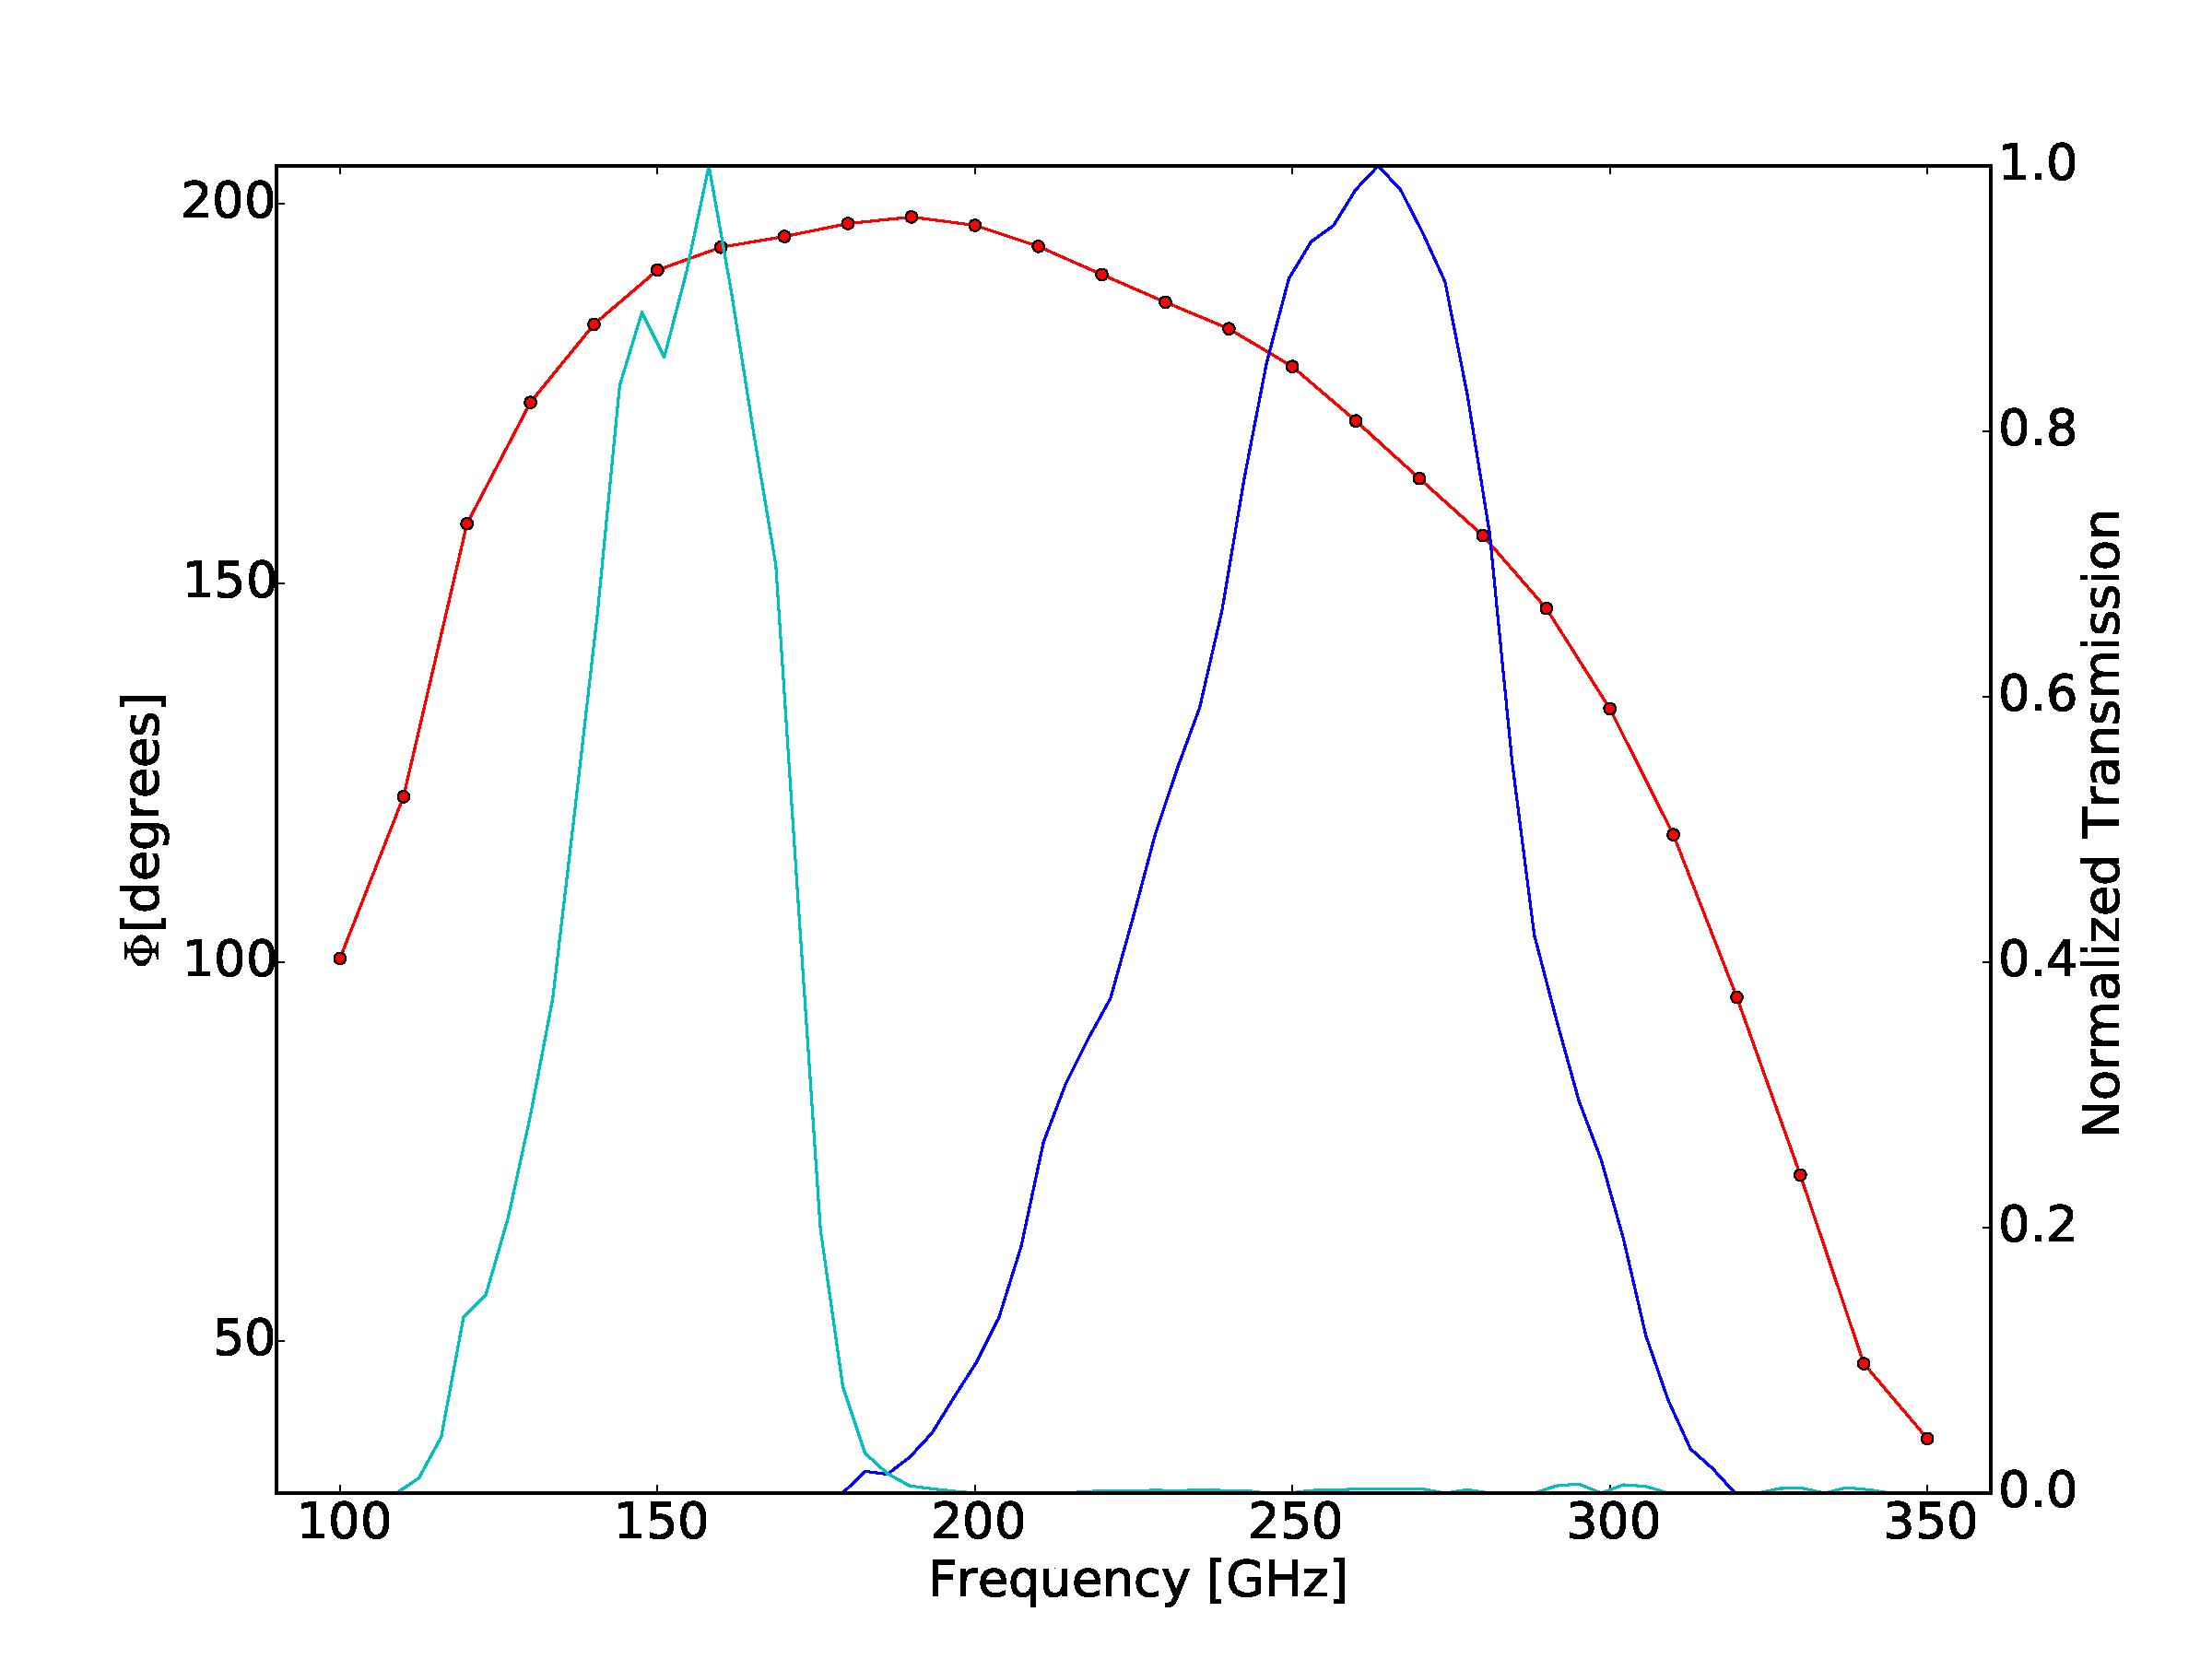
\includegraphics[width=9cm, keepaspectratio]{HWPCardiffMeasurements/phase_shift_angle.pdf}
   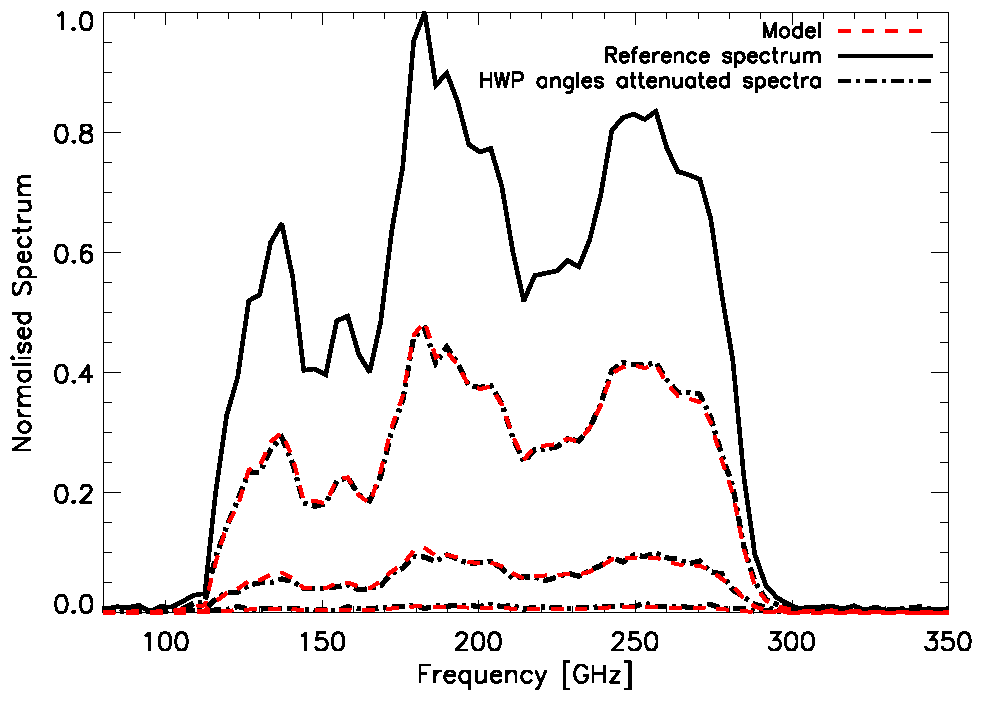
\includegraphics[width=9cm, keepaspectratio]{figures/spectre.pdf}
    \caption{Top: Phase shift angle as a function of frequency for the \nika\ HWP. The transmission for the two \nika\ frequency bands
    at 1 (blue) and 2 (cyan) mm are also plotted for illustration. Bottom: 
    Spectral transmission of the \nika\ HWP for different angles. %with respect to the optical axis.
    The red curve corresponds to the best-fit model for the intermediate angle data. The maximum transmission
    \nico{corresponds} to an angle of $46.8^{\circ}$ \nico{w.r.t.}~the HWP zero
    (optical axis).\nico{Attenuated spectra at $72^{\circ}$, $79^{\circ}$,
      $86.4^{\circ}$ are also shown.}}
        \label{fig:spectre}
  \end{center}
\end{figure}
\begin{figure}
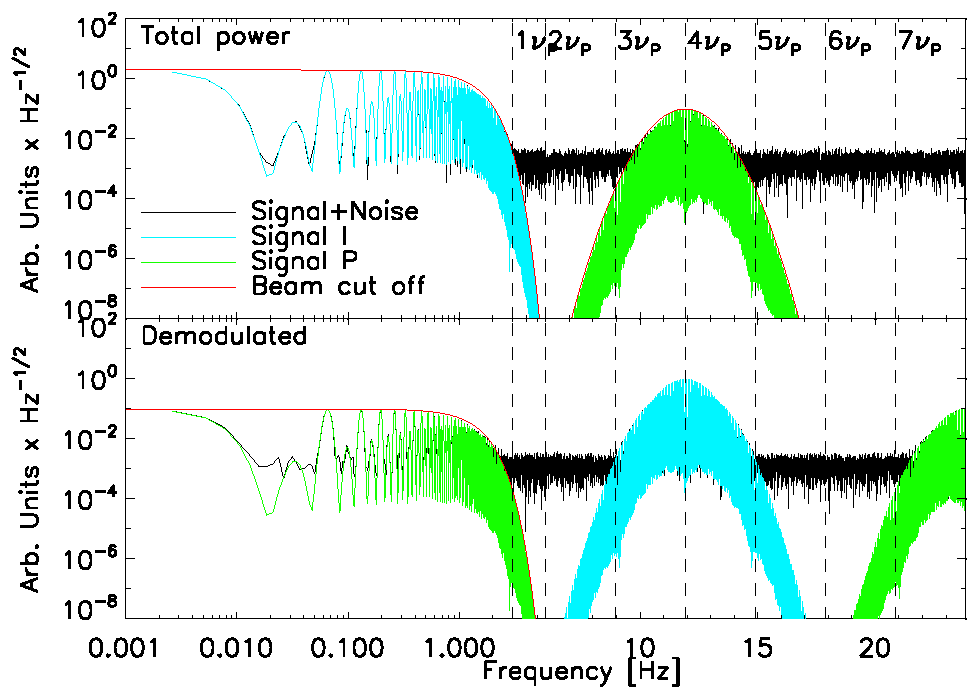
\includegraphics[width=1.\linewidth,keepaspectratio]{figures/toi_simu.pdf}
\caption{The top panel shows the power spectrum of a simulated \nico{**}
  TOI (Time Ordered Informations) for a polarized point source observed under a
  raster scan \nico{with} a continuously rotating HWP facing
  a polarization analyzer. The raw signal plus noise TOI (black) has its total
  intensity content highlighted in cyan and the polarized content in green. The
  polarization signal band is centered on the fourth HWP harmonics while the
  intensity signal band lays at lower frequencies. On the bottom plot, we
  present the TOI after demodulation (see. Sect.~\ref{se:lockin}). We observe
  that half of its Stokes $Q$ content has been put at low frequency while the
  Stokes $I$ content and the remaining polarized contents are shifted at
  frequencies higher than the signal band.}
   \label{fig:toi_simu}
\end{figure}  
%\section{Observation strategy for polarization measurements}
\begin{figure*}
  \begin{center}
  \includegraphics[%
  width=7.5cm, keepaspectratio]{figures/TOI.eps}
  \includegraphics[%
  width=7.85cm, keepaspectratio]{figures/spectre_I_fit.eps}
\caption{TOI (left) and power spectrum (right) of an observation of Orion OMC-1
  for a single KID. Raw data are presented in black and the half wave plate systematic signal (HWPSS) subtracted
  data in green.}
  \label{toi_i}
   \end{center}
   \end{figure*}  
    \begin{figure}
  \begin{center}
    \includegraphics[%
      width=10cm,keepaspectratio]{figures/template_drift.eps}
    \caption{Absolute amplitudes of the four main harmonics of the HWPSS as a function of time. Each point is a measurement of these amplitudes on a chunk of about 30 seconds. The amplitudes show a slow and linear drift in time.}
    \label{time_drift}
  \end{center}
\end{figure}
 \begin{figure*}
   \begin{center}
     \includegraphics[%
       width=6cm,keepaspectratio]{figures/spectre_I_fit_decor.eps}
     \includegraphics[%	
       width=6cm,keepaspectratio]{figures/spectre_Q_fit_decor.eps}
     \includegraphics[%	
       width=6cm,keepaspectratio]{figures/spectre_U_fit_decor.eps}
     \caption{From left to right power spectra of the Stokes $I$, $Q$, $U$ pure
       TOIs (black) after applying the lock-in procedure to the raw data on
       Fig.~\ref{toi_i}.  A bandpass filter ($[0.01,2.9]$~Hz) is applied to
       reject any high frequency noise and half wave plate systematic signal (HWPSS) residual at the fourth
       harmonics. In blue we also show the power spectra after applying the
       decorrelation procedure to the demodulated data.  See
       Sect.~\ref{se:demod_mapmaking} for details. \nico{can we redo these
         pictures with the red fit forced to a constant rather than this
         misleading 1/f ?}}
     \label{spectre_iqu}
   \end{center}
 \end{figure*}


%% of the for each wavelength due to the linear relation
%% between the phase shift and the wavelength. This effect is expected to be quite
%% weak because the HWP is achromatic \citep{moncelsi2014}. First we measured a
%% spectrum with the HWP aligned to its ordinary axis. This corresponds to the
%% maximum signal in which we expect to have no distortion {\color{red} see
%%   comment} of the {\it NIKA}
%% bandpass, as measured in intensity \citep{catalano2014}. This is taken as a
%% reference spectrum. Rotating the HWP we found an attenuation as shown in
%% Fig.~\ref{fig:spectre}, here the maximum transmission is represented by the
%% spectrum at about 46.8$^{\circ}$ $\pm$ 1.8$^{\circ}$ with respect to the HWP
%% zero.

% The polarized transmission is therefore of $\sim$ 100\% in the {\it NIKA} band
% frequency with a polarized transmission loss of 0.6 $\%$ in the 1mm channel and
% of 1.4$\%$ in the 2mm channel.
 
%In the 1mm channel the polarization loss is very low so we consider to work with
%an ideal HWP assuming the $\rho_{pol}$ = 1 in the following data reduction
%analyzis. In the 2mm channel we take into account for the coefficient
%$\rho_{pol}$ in the calibration factor.


\section{Reconstruction of the \nika\ Stokes parameter maps}
\label{data_analysis}

We here describe the specificities of \nika's polarization modulation strategy
and data analysis. We start by giving more details on the fast and continuous
rotation of the HWP and how it impacts the signal. We then present specific
systematics associated to the rotating HWP and the optics, and how we handle
them. 
%We postpone the determination of the absolute polarization angle on the
%sky and of the absolute calibraiton to the following section.

 
\subsection{Polarization modulation with a continuously rotating HWP}
\label{se:lockin}

%: a scan in azimuth at constant elevation and constant speed
%$v$, an elevation step smaller than the beam FWHM, another azimuth scan at this
%new elevation, this sequence being repeated until we have scanned the desired
%sky area. In such a case, the point source signal appears in time domain at
The key aspect for reconstructing polarization with \nika\ is the rotating HWP,
which modulates the input polarization signal.  Thus, we recall here the main
lines guiding polarization modulation by a continously rotating HWP and its
subsequent data analysis. For the sake of clarity, we consider the case of a
polarized point source, which is observed under a classical raster scan strategy
with constant declination while scanning along right ascension $\alpha$ at speed
$\dot{\alpha}$. This type of scan being pseudo-periodical, the Fourier transform
of the detector observed time ordered data (TOI, equivalent to Time Ordered Information) shows peaks at harmonics of the
scanning frequency (Fig.~\ref{fig:toi_simu}), each peak containing the sum of
the unpolarized and polarized fluxes of the source (see
equation~\ref{photoequ}). These peaks are damped by the instrument resolution at
high frequency. The cut off at
high spatial resolution turns into a high temporal frequencies cutoff with
typical Gaussian width $FWHM_\nu = \dot{\alpha}/2\pi FWHM$. This beam cutoff
defines the signal band. According to Eq.~(\ref{photoequ}), when we rotate a HWP
in front of an analyzer, the polarized fraction of the signal is modulated at
four times the mechanical rotation frequency of the HWP. Therefore, this shifts the
polarized content of the signal at higher frequencies and recenters the signal
band around the fourth harmonic of the mechanical rotation of the HWP (see
Fig.~\ref{fig:toi_simu}-top). It is then clear, that a lowpass filter applied to
the data above the beam cutoff and below the polarization signal band will
preserve the unpolarized signal band while rejecting the polarized content and
high frequency noise. We will refer to this type of TOIs as ``pure-$I$''
TOI in the following. To recover the polarization Stokes parameters $Q$
and $U$, we use a demodulation procedure pioneered by \cite{johnson2007}. We
build two reference signals :
\begin{eqnarray}
ref_Q = \cos(2\psi(t) + 4\omega_Pt) \nonumber \\
ref_U = \sin(2\psi(t) + 4\omega_Pt)
\end{eqnarray}
We multiply our TOIs by these reference signals and according
to Eq.~(\ref{photoequ}) obtain {\it e.g.} $Q/2 + I\cos[2\psi(t)+4\omega_Pt] +...$ $Q$
and $U$ terms around the 8th harmonics of the HWP rotation. We have thus
``demodulated'' the $Q$ content of the TOI and brought it back at low
frequencies, while rejecting the $U$ and $I$ content at high frequencies. A low
pass filter above the beam cutoff and below the tail of the modulated intensity
therefore provides a ``pure-$Q$''  TOI (see the bottom panel of
Fig.~\ref{fig:toi_simu}). Equivalently multiplying by
$\sin\left[2\psi(t)+4\omega_Pt\right]$ and filtering we obtain a ``pure-$U$'' TOI.

\subsection{Polarization measurements at the telescope}
\label{polsetup}
The \nika\ polarization setup at the telescope was similar to the one in the
laboratory as shown on the right panel of Fig.~\ref{polarsetup}.  The HWP and
analyzer were placed in the same mount facing the cryostat window in the optical
axis of the Nasmyth cabin. Thus, the polarization reference frame was defined
perpendicularly to the optical axis in Nasmyth coordinates. \nico{We should
  subtract this sentence it adds confusion: no plot is showing it, nobody but us doing the
  commissionning actually cares...: ``Note that the image at the Nasmyth cabin
  is rotated by 45.4 degrees with respect to the sky.''} This rotation is
accounted for when reconstructing polarization on sky coordinates.
% The analyzer was slightly tilted (about 10 degrees) with respect to the HWP to avoid standing waves.

During polarization observations the HWP was continuously rotated to modulate
the input polarization signal as discussed in Sect~\ref{se:lockin}. The optimal
HWP rotation speed is constrained by several factors including scanning speed
and the scale of atmospheric variations. Usual scanning speeds for \nika\ were
$\sim$ few tens of arcsec/s. Atmospheric turbulence and variations
across the scan \nico{transform} into $1/f$ like noise with typical knee frequency
below 1-2~Hz for reasonable atmospheric conditions \nico{, as illustrated on
  Fig.~\ref{toi_i} that shows} the measured raw TOI (black curve) for a single detector as a
function of sample number (left) and \nico{its} corresponding power spectrum
(right). \nico{**}
%Atmospheric emission fluctuations are observed as low frequency drifts
%in the TOI that correspond to a $1/f$ like structure in the power
%spectrum.
In addition to the atmospheric noise a subdominant detector
correlated-noise component had been found in the \nika\ data and identified as
electronic based noise.
%Electronics noise becomes
%subdominant above 1~Hz as well {\color{red} exact value TBC}. 
Rotating the HWP such that 4 times its rotation speed places the polarization
signal well above 2~Hz permits a natural rejection of these two major noise
components. If the rotation is also fast compared to the scanning speed and the
angular resolution, the three Stokes parameters can be derived
quasi-simultaneously, thus rejecting further residual low frequency
drifts. Finally, a fast rotation places possible parasitic signals at harmonics
of the rotation frequency outside the signal band (see Sect.~\ref{se:hwpss} for
more details). Both the polarization modulation and parasitic signals can be
clearly observed on Fig.~\ref{toi_i} as high frequency peaks in the TOI spectrum
at harmonics of the HWP rotation frequency. \nico{A fast} rotation sets tight mechanical
constraints on the stepper motor and impose a faster data acquisition with
respect to unpolarized observations. That is why we chose, as discussed above,
to acquire data at 47.7~Hz, rotate the HWP at 2.98~Hz and to limit our scanning
speed to 26~arcsec/s. This provides 5 measures of $I$, $Q$ and $U$ per FWHM,
well within the Nyquist limit, even at a LEKID timeline level. Each of these 5
measures results from the combination of four data samples taken at four
different HWP angles. To conclude, we are then able to reconstruct the Stokes
parameters per detector, with high spatial and temporal redundancy and to reject
atmospheric noise from the polarization signal band.
\subsection{Systematic HWP synchronous signal correction}
\label{se:hwpss}
Imperfections of the HWP modulate the background and lead to a strong
additional parasitic signal, highly peaked at harmonics of the HWP rotation
frequency $\nu_P$ as shown on the left panel of Fig.~\ref{toi_i}. Such a HWP
Synchronous Signal (HWPSS) was previously observed by Maxima \citep{johnson2007}
and EBEX \citep{ebex}, although the HWP driving mechanisms were
  different. Like them, we find that the signal is well fitted by a sum of
harmonics of the HWP rotation frequency, $\nu_P$ with amplitudes slowly and
linearly drifting. This is illustrated in Fig.~\ref{time_drift} where we plot
the time variation of the cosine $A_n$ (red) and sine $B_n$ (blue) component
amplitudes of the first four harmonics of the HWP rotation frequency along a scan of Uranus. To derive these amplitudes, we use a simplified model of Eq.~(\ref{eq:hwpss}) to fit only the constant part of amplitudes $A_n$ and $B_n$ over chunks of 30 seconds. We observe that the relative
variation is at most $2\times 10^{-3}$ Jy/s, mainly dependent on the background (Stokes $I$). 
We therefore model this additional parasitic signal as a Fourier series of 
the harmonics of the HWP rotation frequency
\begin{eqnarray}
HWPSS(t) &= \sum_{n=1}^{8}& (A_n^{0}+ \epsilon_{A_n}t)\cos n\omega_Pt\nonumber\\
&& +(B_n^{0}+\epsilon_{B_n}t)\sin n\omega_Pt
\label{eq:hwpss}
\end{eqnarray}
where
\begin{eqnarray}
A_n = A_n^0 + \epsilon_{A_n}t \nonumber \\
B_n = B_n^0 + \epsilon_{B_n}t
\end{eqnarray}
We consider up to 8 harmonics of $\nu_{P}$ and explicitly include a linear variation of the
amplitude coefficients both for the sine and cosine components when we fit this model on data.
%We collect all samples of a kid into a vector ${\bf v}$, build a matrix $T$
%whose columns are $\cos n2\pi\nu_Pt$, $t\cos n2\pi\nu_Pt$, $\sin n2\pi\nu_Pt$
%and $t\sin n2\pi\nu_Pt$. We then perform a maximum likelihood fit giving the
%same weight to all samples ${\bf a} =
%(T^TT)^{-1}T^T{\bf v}$ to derive ${\bf a}$, a vector containing amplitudes $A_n$,
%$B_n$ and $\epsilon_{A_n}$ and $\epsilon_{B_n}$. With this amplitudes in hand,
%we can build a model of the HWPSS in the kid timeline and subtract it.
We perform a simple linear fit of the previous model to the full calibrated and
opacity corrected (see Sect.~\ref{se:calib} for details) raw TOI to derive the
best-fit amplitude coefficients. With these coefficients in hand, we
construct a template of the HWPSS which is then subtracted from the raw
calibrated TOI. An illustration of this procedure is shown in the left panel of
Fig.~\ref{toi_i} where the raw TOI is shown before (black) and after (green)
subtraction of the HWPSS template. Equivalently, the right panel of the figure
presents the power spectrum of the raw TOI before (black) and after (green) the
subtraction of the HWPSS template. Thanks to this procedure, the
HWPSS residuals are reduced to the noise level.
%We could in principle improve this fit by using only data 
%samples far from the source when possible. However, the HWPSS 
%is much stronger than the brightest astronomical signals we observe, and not sky
%synchronous. We thus found that it did not make any difference to take this
%extra precaution, and as far as this technical run is concerned, we did not
%apply this masking. {\color{red} we need to conclude this Sect. by a plot
%showing how well this model subtracts the ``true'' HWPSS. We must also repeat
%that we actually care only about effects around $4\nu_P$}\\
\subsection{\nika\ demodulation procedure and map making}
\label{se:demod_mapmaking}
%In order to extract the polarized signal from the unpolarized foreground we use
%the modulation/demodulation technique: by means of a polarization modulator, the
%HWP in our case, the polarized component of the incoming radiation is modulated
%at a precise frequency.
%A total power detector such as a LEKID or a bolometer, hit by a
%  polarized light, measures a combination of the three Stokes parameters. The
%  relative weights of the Stokes parameters are then a function of the
%  orientation of the incoming polarization and at least three different
%  orientations are needed to separate $I$, $Q$ and $U$ in principle. The
%  rotation of the HWP in front of the analyzer provides this rotation following
%  Eq.~(\ref{signal_polar}).
After subtraction of the HWPSS, we use the lock-in procedure described in
Sect.~\ref{se:lockin} to separate the raw TOI per KID into pure Stokes $I$,
$Q$ and $U$ TOIs. These TOIs are decorrelated from a common mode to remove the
residual atmospheric and electronic noise, and then projected into Stokes $I$, $Q$ and
$U$ maps.  We use the same decorrelation procedures developed for the
intensity-only \nika\ observations \citep[see][for
 details]{adam2014,catalano2014}. In particular we use a common mode decorrelation masking the source
 and using only the pixels outside the source to decorrelate.
 A low pass filter is also applied to the pure
Stokes $I$, $Q$ and $U$ TOIs to reject high frequency noise. The frequency
cutoff is set slightly below the HWP rotation frequency.  For the projection we
use an inverse noise weighting procedure and account for instrumental flags
indicating unreliable data samples or detectors \citep[see][for details]{adam2014,catalano2014}.
In the case of the $Q$ and $U$ maps, this map
making procedure is nearly optimal map making because the noise is
expected to be nearly white in the pure Stokes $Q$ and $U$ TOIs. This is
illustrated in Fig.~\ref{spectre_iqu} where we present in black the power
spectra of the pure Stokes $I$, $Q$ and $U$ TOIs obtained by applying the lock-in
procedure to the raw TOI of Fig.~\ref{toi_i}. We observe that the power
spectra of the pure Stokes $Q$ and $U$ TOIs are nearly flat indicating, as
expected, a significant, although not complete, reduction of the contribution from
atmospheric fluctuations that shows like a $1/f$ like component on a pure $I$
TOI.
%%combination of the atmospheric and electronic noise.  Fitting the power spectra
%%of the pure Stokes $I$, $Q$ and $U$ TOIs to a model of the form $ P(f) = k
%%f^{\beta}$ we find negligible $1/f$ like components for $Q$ and $U$ and a
%%dominant one for $I$.

The best-fit power spectrum models are presented in red on
Fig.~\ref{spectre_iqu}. Using simulations we have proven that the residual $1/f$
like component in $Q$ and $U$ is consistent with residual atmospheric emission
induced by intensity to polarization leakage as discussed in
Sect.~\ref{sec:polleak}. We also show in blue the power spectra after applying
the decorrelation procedure. This leads to a significant reduction of the $1/f$
like noise in the pure Stokes $I$ TOI power spectrum and of the residual low
frequency tail on the pure Stokes $Q$ and $U$ TOIs.
	
%% This technique allows the quasi-simultaneous measurements of the three Stokes
%% parameters ($I$, $Q$, $U$) on a given sky position. The polarized signal is
%% expected modulated at four times the mechanical rotation frequency of the HWP.
%% The polarized signal is extracted using demodulation procedure detailed in
%% \citep{johnson2007}.

%% The expected signal measured by a KID $k$ is:
%% \begin{equation}
%%  m_{k} =  \frac{1}{2}\{I + {\rho}_{\rm pol}[Q\cos(4{\omega}t + 2{\alpha}_{\rm Sky}(p_{\rm t})) +  U\sin({4{\omega}t} + 2{\alpha}_{\rm Sky}(p_{\rm t}))]\}
%%  \label{signal_polar}
%%  \end{equation}
%%  where ${\rho}_{\rm pol}$ is the polarization efficiency


 
\subsection{Absolute calibration and inter-calibration}
\label{se:calib}

Absolute calibration is performed in the same way as for the intensity only
\nika\ observations \citep{adam2014,catalano2014}. We use Uranus as our main
absolute flux calibrator and compute calibration factors per KID by fitting a 2D
Gaussian to the data. We take the measured FWHMs of 12~arcsec at 1.15~mm and
18.2~arcsec at 2.05~mm. For the data presented in this paper, we have 15\% uncertainty on
absolute calibration at 1.15~mm and 10\% at 2.05~mm \citep{catalano2014}.  
The standard deviation of the flux distribution on Uranus gives directly the calibration 
error associated to the estimation of point sources flux values.
After calibration, the data
are given in units of Jy/beam.  We also correct the raw data from atmospheric
absorption using the \nika\ instrument as a taumeter following the procedure
described in~\cite{catalano2014}. The procedure is based on the fact that the
response - the change in resonant frequency for a given change in absorbed power
- of KIDs is linear and it is a constant property of each detector.

\subsection{Instrumental polarization and leakage}
\label{sec:polleak}
%% {\color{green} to be rephrased and placed somewhere else: As we have discussed
%%   above the power spectrum of the TOIP is consisting with a flat spectrum. The
%%   negative and positive beam observed in the leakage maps compensate each other
%%   and smooth the effect.  Taking a convolution between the atmospherical spread
%%   signal, the Stokes intensity $I$ map with the characteristic 1/f component of
%%   noise, and the leakage beam in $Q$ and $U$ we found that the two component
%%   compensation drowning the effect in a white noise.}
Like most authors, we define instrumental polarization as the ability of the
instrument to convert incident unpolarized total power into a polarized
signal. This conversion can then take various forms, as we describe in this
section. To estimate the level of instrumental polarization at the telescope we
repeatedly observed Uranus, which is unpolarized (\cite{polka_apex} find a
polarization of $\sim 0.1 \%$)\nico{added brackets here}, and bright (47.2~Jy at 1mm, 16.4~Jy at
2.05mm). It has an apparent diameter at the time of observations of 3~arcsec and
can then be considered as a point source compared to our
beams. Fig.~\ref{fig:uranus_lkg} shows Stokes $I$, $Q$ and $U$ maps of Uranus in
Nasmyth ({\it i.e.}~cabin) coordinates at 1 and 2.05 mm in panels (a) and (b),
respectively.  For each panel the top row shows the raw \nika\ maps after
projection of the decorrelated pure Stokes $I$, $Q$ and $U$ TOIs. We observe a
significant signal in $Q$ and $U$ that indicates a non zero level of
instrumental polarization. We identify mainly a bipolar pattern, partially
consistent between the two bands, with a peak to peak amplitude at the level of
3\% of the total intensity peak. Such an effect has already been observed on
other experiments, (e.~g.~\citep{thum2008} and \citep[][]{2015ApJ...806..206B}).
We have performed a large number of observations of Uranus at different
elevation angles. From these observations we have concluded that the observed
leakage effect is fixed in Nasmyth coordinates.  \\
\begin{figure*}
  \begin{center}
\setlength{\unitlength}{\columnwidth} 
\begin{picture}(2,2.5)
%Uncorrected 1 mm
    \put(0.05,2.48){(a) 1.15 mm raw (top row) and leakage corrected (bottom row) Stokes $I$,$Q$ and $U$ maps.}
     \put(0,1.85){ \includegraphics[width=0.33\linewidth,keepaspectratio]{figures/Uranus_I_map.eps}}
     \put(0.7,1.85){\includegraphics[width=0.33\linewidth,keepaspectratio]{figures/Uranus_Q_map.eps}}
       \put(1.4,1.85){\includegraphics[width=0.33\linewidth,keepaspectratio]{figures/Uranus_U_map.eps}}
 
 %Corrected 1 mm
     
      \put(0,1.25){\includegraphics[width=0.33\linewidth,keepaspectratio]{figures/Uranus_I_map_corr.eps}}
     \put(0.7,1.25){\includegraphics[width=0.33\linewidth,keepaspectratio]{figures/Uranus_Q_map_corr.eps}}
     \put(1.4,1.25){ \includegraphics[width=0.33\linewidth,keepaspectratio]{figures/Uranus_U_map_corr.eps}}

%Uncorrected 2 mm
  
    \put(0.05,1.22){(b) 2.05 mm raw (top row) and leakage corrected (bottom row) Stokes $I$, $Q$ and $U$ maps.}

      \put(0,0.6){\includegraphics[width=0.33\linewidth,keepaspectratio]{figures/Uranus_I_map_2mm.eps}}
      \put(0.7,0.6){\includegraphics[width=0.33\linewidth,keepaspectratio]{figures/Uranus_Q_map_2mm.eps}}
     \put(1.4,0.6){\includegraphics[width=0.33\linewidth,keepaspectratio]{figures/Uranus_U_map_2mm.eps}}
  %Corrected 2 mm
      \put(0,0){\includegraphics[width=0.33\linewidth,keepaspectratio]{figures/Uranus_I_map_2mm_corr.eps}}
     \put(0.7,0){\includegraphics[width=0.33\linewidth,keepaspectratio]{figures/Uranus_Q_map_2mm_corr.eps}}
     \put(1.4,0){\includegraphics[width=0.33\linewidth,keepaspectratio]{figures/Uranus_U_map_2mm_corr.eps}}

\end{picture}

  \caption{ Uranus Stokes $I$, $Q$ and $U$ maps in Nasmyth coordinates at 260
    GHz (a) and 150 GHz (b) before and after leakage correction. After the
    leakage correction, we are left with a residual instrumental polarization below 1\% (0.7 \% at 1.15 mm and 0.6 \% at 2.05 mm).}
    %below 1\% that is straightforward to take into account.}
  \label{fig:uranus_lkg}
  \end{center}
\end{figure*}
\noindent Although we still lack a convincing physical interpretation
 of the observed signal, we can model it as leakage from total intensity $I$ into
 $Q$ and $U$, and write the observed Stokes parameters in Nasmyth
 coordinates as
 \begin{eqnarray}
 \hat{I}_{N}  & = & B_{I} * I_{N} + {\cal{N}}_{I} \nonumber \\
 \hat{Q}_{N}  & = & B_{I} * Q_{N} + {\cal{L}}^{IQ}_{N} * I_{N} + {\cal{N}}_{Q} \nonumber \\
 \hat{U}_{N}  & = & B_{I} * U_{N} + {\cal{L}}^{IU}_{N} * I_{N} + {\cal{N}}_{U} 
 \label{eq_leak}
 \end{eqnarray}
 where $I_{N}$, $Q_{N}$ and $U_{N}$ are the original sky Stokes parameters in
 Nasmyth coordinates. $B_{I}$ represents the \nika\ response pattern and $*$ denotes
 spatial convolution. The different noise contributions discussed above are
 accounted for in ${\cal{N}}_{I,Q,U}$ \nico{please use $N$ rather $\cal{N}$ and
   $\cal{B}$ rather than $B$ to
   distinguish a convolution kernel from a map}. Finally, we model the leakage term as the
 convolution of the original intensity map with response pattern like kernels
 ${\cal{L}}^{IQ}_{N}$ and ${\cal{L}}^{IU}_{N}$ for $Q$ and $U$,
 respectively. These two kernels are directly estimated from the $Q_{N}$ and
 $U_{N}$ maps of Uranus presented in Fig.~\ref{fig:uranus_lkg}, which, as
 discussed above can be considered as a point source. Note that we assume here
 no modification of the intensity signal and account for any loss of power at
 the calibration stage. \\
 
 %We denote quantities unaffected by any beam with a $_0$ index and with a $^N$ superscript,
 %quantities evaluated in Nasmyth coordinates. Like in Sect.~\ref{se:pol_module},
 %$\psi$ is the polarization observation angle that accounts for both the HWP
 %angle and the parallactic angle. Leaving noise aside for the sake of
 %readability, we model the noise less measurement of a kid $k$ at time $t$ such
 %as the sum of the signal convolved by the instrumental main beam $B_I$ and of an
 %extra leakage term from the signal intensity into $Q$ and $U$:
 %\begin{eqnarray}
 %S_k &=& B_I * (I^N_0 + Q^N_0\cos2\psi + U^N_0\sin2\psi) \nonumber \\
 %       &&+ L_{IQ}*I^N_0\cos2\psi + L_{IU}*I^N_0\sin2\psi,
 %\label{eq_leak}
 %\end{eqnarray}
 
 %where $*$ denotes convolution. As Uranus can be considered as a point source
 %with respect to the \nika's angular resolution, the $Q^N$ and $U^N$ maps give
 %directly the $L_{ IQ}$ and $L_{ IU}$ beams, up to an absolute calibration factor
 %that is straightforward to scale by comparing to the $I$ map. All that is needed
 %now to subtract the leakage terms from the measurements is an estimate of
 %$I^N_0$. While we cannot deconvolve the observed $I$ map from the instrumental
 %beam $B_I$ with perfect accuracy, this is actually not needed since $I^N_0$ must
 %be convolved back by $L_{IQ}$ and $L_{IU}$. This sets a scale in Fourier space
 %up to which division by the instrumental beam $B_I$ remains accurate enough
 %compared to knowledge on $B_I$ and on map noise, and above which multiplication
 %by the leakage beams ensures a regularizing damping. We thus summarize our
 %correction process as:
 
 \noindent To correct for this leakage effect we have developed a dedicated algorithm
 based on the above model.
 \begin{enumerate}
 \item With the demodulation and projection techniques presented in
   Sect.~\ref{data_analysis}, we build maps of Stokes $I$, $Q$ and $U$ of the
   observed signal in equatorial coordinates. These maps can be the result of
   multiple observation scans to obtain the best possible signal to
   noise. We only need the $I$ map in the following to derive the leakage signal that we want to subtract.
 \item Rotate the $I$ map into Nasmyth coordinates to obtain $\hat{I}_N$ for
   a given scan. The needed rotation angle, which is the combination of the
   elevation and the parallactic angles, varies along the scan. However, we find
   that not accounting for this variation leads to negligible differences.
 \item Build Fourier space convolution/deconvolution kernels of the form
   ${\cal{L}}_{IQ}/B_I$ and ${\cal{L}}_{IU}/B_I$ from observations of
   Uranus.
 \item Multiply the Fourier transform of $I^N$ by the above kernels 
   and transform the result back into real space to build maps of leakage from $I$ into $Q$ and $U$.
 \item Deproject the obtained maps with the actual scanning strategy to produce $Q$ and $U$ TOIs that
  are then subtracted from the decorrelated pure Stokes $Q$ and $U$ TOIs presented in Sect~\ref{se:demod_mapmaking}.
 \item Project these corrected TOIs onto final maps following the same map making
   procedure as in Sect~\ref{se:demod_mapmaking}.
 \end{enumerate}
 
 In Fig.~\ref{fig:uranus_lkg} the bottom rows of panels (a) and (b) show the
 final Nasmyth coordinate Uranus Stokes $I$, $Q$ and $U$ maps after leakage
 correction using the above algorithm. Note that to compute the leakage kernels
 we use a set of independent Uranus observations to cross check the efficiency of
 the procedure.  We observe that after leakage correction the residual leakage in
 the $Q$ and $U$ maps of Uranus drops below 1 \%. We now see a residual
 signal that we interpret as ``straightforward'' instrumental polarization,
 {\it i.e.} an induced polarization directly proportional to $I$. This instrumental
 polarization is below 1\% for both $Q$ and $U$, and is removed
 by subtracting the relative fraction of the total intensity map from
 our polarization maps.

We apply this correction to polarized objects as well. The top row of
Fig.~\ref{3c273_ex} shows the \nika\ Stokes $I$, $Q$ and $U$ maps at 2.05 mm
of the quasar 3C273 before leakage correction. We clearly see in the $Q$ and $U$
maps a dipolar structure similar to the one observed on the Uranus maps. The
bottom row of the figure presents the leakage corrected maps, which show no
residual dipolar structure but slightly increased noise contribution. Indeed,
the division by $\tilde{B_I}$ boosts the signal on small angular scales and therefore the
noise, but the damping of ${\cal{L}}_{IQ}$ compensates and ensures
regularization. For a single observation with fixed scanning direction, we
observe a small increase of the low frequency noise (striping) as observed on
Fig.~\ref{3c273_ex}. This is then compensated by the combination of multiple
scans in different orientations. 
 \begin{figure} 
  \begin{center}
     \includegraphics[%
      width=1.3\linewidth,keepaspectratio]{figures/pipeline_scheme_v2.eps}
\caption{Schematic view of the main procedures of the data processing pipeline from raw data to sky maps.}
\end{center}
\label{fig:scheme_pipe}

\end{figure}
 \subsection{Summary of data processing pipeline}\label{se:sumpipe}
 Fig.~\ref{fig:scheme_pipe} presents a schematic view of the main procedures used
 to convert the raw \nika\ data into leakage corrected Stokes $I$, $Q$ and $U$
 maps. The main steps are
 \begin{enumerate}
 \item Read raw data
 \item Reconstruct the position of the HWP and the corresponding angle with respect to the zero reference
 \item  Compute absolute calibration and correct for atmospheric absorption
 \item  Apply a basic de-glitching algorithm to remove spikes on the raw \nika\ TOIs
 \item  Reconstruct and subtract the HWPSS
 \item  Apply lock-in procedure to the raw \nika\ TOIs to build pure Stokes $I$, $Q$ and $U$ TOIs
 \item  Apply the decorrelation procedure to the pure Stokes $I$, $Q$ and $U$ TOIs
 \item  Apply a basic de-glitching algorithm to remove spikes on the pure Stokes $I$, $Q$ and $U$ TOIs
 \item  Apply the leakage correction algorithm to the decorrelated pure Stokes $I$, $Q$ and $U$ TOIs
 \item  Apply the map making procedure to the decorrelated and leakage corrected pure Stokes $I$, $Q$ and $U$ TOIs
 \item Project the cleaned TOIs into maps.
 \end{enumerate}
 
 %%==========================================================================================
 
 
 
 %% In real conditions there is an additional parasitic signal at harmonics of 1{$\omega$}, 2{$\omega$}, 3{$\omega$} etc, due to imperfections of the HWP. Furthermore, the atmospheric and electronic noise need to be taken into account. 
 %% Thus Eq. (\ref{signal_polar}) reads:
 %% \begin{eqnarray}
 %%  m_{k} &=& \frac{1}{2}\{I + {\rho}_{ pol}[Q\cos(4{\omega}t + 2{\alpha}_{\rm Sky}(p_{\rm t})) + Usin({4{\omega}t} \nonumber \\
 %%  	  &+& 2{\alpha}_{Sky}(p_{\rm t})]+ S_{\rm parasitic} ({\omega}t, 2{\omega}t, 3{\omega}t, ...)\} \nonumber \\
 %% 	  &+& {\rm atmosphere} + {\rm noise}_{\rm detector}
 %%  \label{pol_eq}
 %%  \end{eqnarray}
 %%  where $p_{\rm t}$ represents the pixel observed at time $t$ and ${\alpha}_{\rm Sky}$ the angle between the telescope reference frame and the local meridian on the sky. 
 %% The angle ${\alpha}_{\rm Sky}$ is measured from north to east in the equatorial system as  ${\alpha}_{\rm Sky} = {\tau} - {\epsilon} - {\eta}$,
 %% where ${\epsilon}$ represents the elevation, ${\eta}$ the parallactic angle, and ${\tau}$ = 45.54$^{\circ}$ is the tilt of the switch mirror of the Nasmyth system along the elevation axis, which creates an angular offset of the image of the sky on the detectors arrays. 	
 %% 
 
 
 
 %%  \section{Data analysis}\label{sec:pipeline}
 %% In order to calibrate, filter, and project data onto sky maps we developed a
 %% dedicated reduction pipeline based on the intensity one described in
 %% \citep{catalano2014, adam2014}. The main steps of the processing consist of:
 %% \begin{itemize}
 %% \item read data time ordered information (TOI): data ordered per kid and regularly sampled with time.
 %% \item TOI calibration: the absolute calibration is applied to these TOIs and an
 %%   atmospheric absorption correction performed. The planet Uranus is the primary
 %%   calibrator for the {\it NIKA} absolute calibration. The calibration factor is
 %%   derived by fitting a Gaussian of fixed angular size on the reconstructed maps
 %%   of Uranus \citep{catalano2014}. The sky maps are corrected for the atmospheric
 %%   contribution rescaling the observed signal by what that would be obtained in
 %%   the absence of the atmosphere. This is achieved via the elevation scan
 %%   technique (\emph{skydip}).
 %% 
 %% The {\it NIKA} atmospheric calibration consist in measuring the variation in the
 %% resonance frequencies of the detectors versus the airmass via elevation scans
 %% (\emph{skydip} \citep{dicke}) from 65 to 20 degrees above the horizon. This
 %% procedure permits to use {\it NIKA} instrument itself as a tau-meter
 %% \citep{catalano2014}.
 %% \item atmospheric and electronic noise decorrelation: depending on the
 %%   scientific target, two basic decorrelation methods are used, 1) a dual-band
 %%   decorrelation using a specific channel to obtain a template of the atmospheric
 %%   emission and 2) a single-band decorrelation where a sky noise TOI template is
 %%   produced by averaging all TOIs of a single array. In both cases we mask the
 %%   astrophysical source to select the pixels far from the source to reconstruct
 %%   the subtraction template (common mode).
 %% \item map-making: TOIs from different detectors of a same frequency band are projected into a single map using a simple coalition. 
 %% 
 %% \end{itemize}
 
 
 % PIPELINE POLAR
 %% \subsection{polarization specific data analysis}\label{sec:polar_pipe}
 %% 
 %%   \begin{figure}
 %%   \begin{center}
 %%   \includegraphics[%
 %%   width=1.\linewidth,keepaspectratio]{figures/Residual.pdf}
 %% \caption{ HWP template amplitudes residual after linear fit subtraction for a KID and all scans of 3C 286.}
 %%   \label{residual}
 %%   \end{center}
 %%   \end{figure}
   
 %%    \begin{figure}
 %%   \begin{center}
 %%   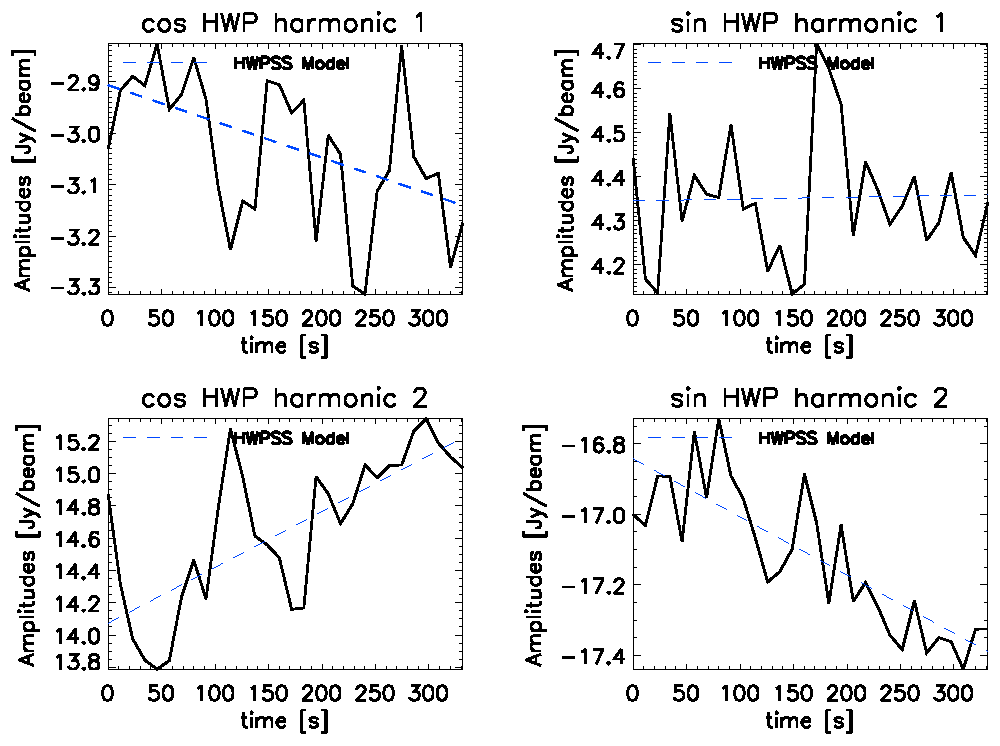
\includegraphics[%
 %%   width=1.\linewidth,keepaspectratio]{figures/ampl_model.pdf}
 %% \caption{ HWPSS template model (dotted blue lines), amplitudes fitted (black line) for a KID and 30 chunk of a scan of 3C 286.}
 %%   \label{ampl_model}
 %%   \end{center}
 %%   \end{figure} 
  
 %%In order to analyse the polarized data output we have developed a dedicated
 %%polarization data reduction pipeline. $I$, $Q$, $U$ Stokes parameters maps in
 %%sky coordinates are constructed by applying the following steps
 %%
 %%\subsubsection{Construct the template of the HWP modulation and removal of parasitic signal.} 
 %%
 %%
 %%%Given a linear polarizing grid aligned with the +$Q$ state and a constant input polarization state, 
 %%As discussed above the polarized power transmitted varies as a sinusoid with
 %%angular frequency 4$\omega$, with amplitude $\propto$ $\sqrt{Q^2 + U^2}$ and
 %%phase $\phi$ $\propto$ $arctan(U/Q)$.
 %%
 %%To have the polarized signal we extract this 4$\omega$ sinusoid component from
 %%the signal recorded by a detector and reconstruct the incident $Q$ and $U$
 %%states for making maps.
 %%
 %%Unfortunately the rotation of the HWP does not simply modulate optical
 %%polarization signals into the detector timestream as sidelobes of
 %%4$\omega$. Defects in the HWP or non-uniformities in its motion can be expected
 %%to generate signals in the detector timestreams at arbitrary harmonics of its
 %%rotation frequency.
 %%
 %%They are stationary in time, and thus appear as spikes in a signal period, which
 %%can be completely described in terms of harmonic number, phase, and
 %%amplitude. The periodic signal that is the combination of these harmonic terms
 %%is called the HWP template.
 %% 
 %%%We fit this signal before proceeding with further analysis. 
 %%Thanks to the synchronization of the detector KID with the acquisition software we can reconstruct the HWP rotation angle and we model the HWP-synchronous signal (HWPSS) \citep{johnson2007} as:
 %%
 %%\begin{eqnarray}
 %% <h_{i}> &=& \sum\limits_{i=1}^N A_i cos(i\omega_{i}) + B_i sin(i\omega) \nonumber \\
 %% 	     &+& A_{i}^{'} t cos(i\omega_{i}) + B_{i}^{'} t sin(i\omega_{i})
 %% \label{hwpss}
 %% \end{eqnarray}
 %% A, B, A$^{'}$, B$^{'}$ represent the amplitudes of N = 9 harmonics considered. We call this estimator $<h_i>$ the HWP template. 
  
 %% To probe the stationarity of the harmonics with time we plot in
 %% Fig.~\ref{time_drift} the ratio between the linear fit coefficients estimated on
 %% the amplitudes variations with time and the HWP template amplitudes fitted $A$,
 %% $B$ reconstructed by the Eq.~\ref{hwpss}. This figure show the percentage HWP
 %% template harmonics variation of $\sim$ 10$^{-3}$. The weak drift in time permits
 %% to assume constant the content of this parasitic signal; the data are cleaned by
 %% the subtraction of the template reconstructed.
 
 %We also observe a harmonics total power content correlated to the opacity
 %variation at 1mm channel, which is more affected by the atmospherical background
 %variation. This correlation is shown in
 %Fig.~\ref{ampl_opac_1mm}. Fig.~\ref{ampl_opac_2mm} shows the harmonics total
 %power content for the 2mm channel observations.
  
 % \begin{figure}
 %  \begin{center}
 %  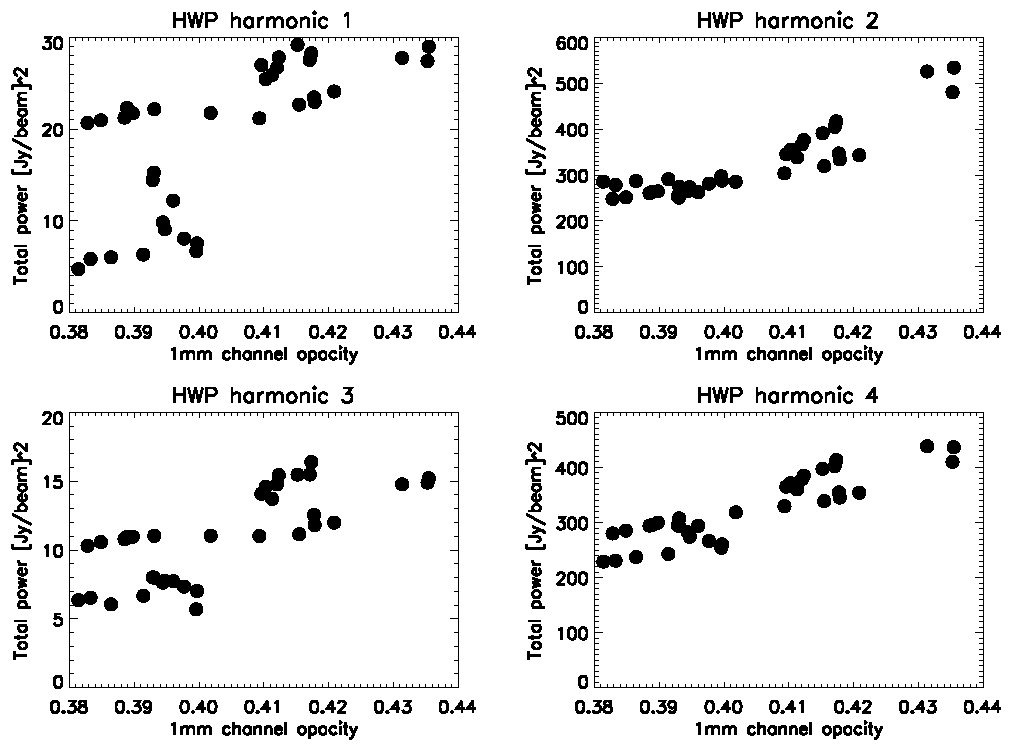
\includegraphics[%
 %  width=1.\linewidth,keepaspectratio]{figures/amplitudes_vs_opacity_1mm.pdf}
 %\caption{ Total power content for four harmonics of the HWP. The plots represent a KID of the 1mm matrix and the monitoring of the HWP template amplitudes for the quasar 3C 286 during three days of observation.}
 %  \label{ampl_opac_1mm}
 %  \end{center}
 %  \end{figure}
     
 %  \begin{figure}
 %  \begin{center}
 %  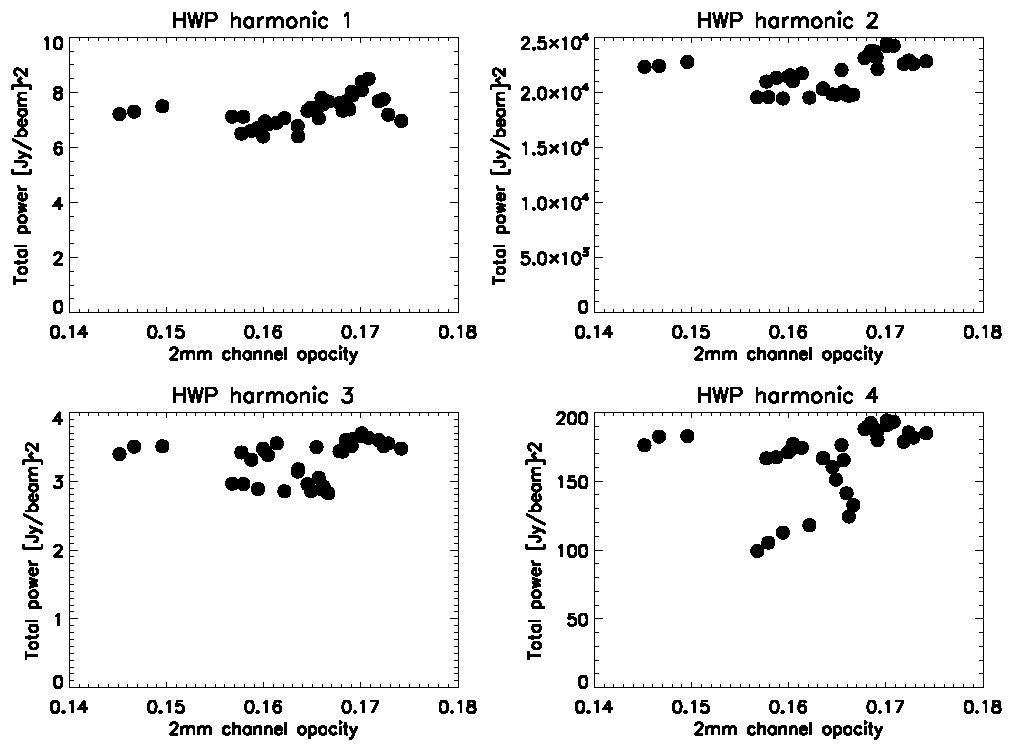
\includegraphics[%
 %  width=1.\linewidth,keepaspectratio]{figures/amplitudes_vs_opacity_2mm.pdf}
 %\caption{ Total power content for four harmonics of the HWP. The plots represent a KID of the 2mm matrix and the monitoring of the HWP template amplitudes for the quasar 3C 286 during three days of observation.}
 %  \label{ampl_opac_2mm}
 %  \end{center}
 %  \end{figure}
 
  
 %% It is built to include terms linear in time to allow for the template amplitude
 %% to drift in time which fit quite well the observed drift; the variations in the
 %% HWP rotation frequency are naturally considered because the sinusoidal terms are
 %% functions of the HWP orientation angle, not of time.
 %% 
 %% The procedure used in the data reduction software returns the HWP template
 %% fitted in order to subtract it from the measured signal $m_k$, see
 %% Eq.~\ref{signal_polar}.
 %% 
 %% Fig.~\ref{toi_i} (left) shows a timeline for a KID of Orion OMC-1 observation
 %% scan, the raw data (black) are atmospheric turbulence affected with a modulated
 %% parasitic synchronous signal at all harmonics of the mechanical rotational
 %% frequency $\omega$, the blue line represents the raw data subtracted for the
 %% synchronous signal template HWPSS.
 %% 
 %% A chunk of the timeline in Fig.~\ref{toi_i} (left) is shown in Fig.~\ref{toi_i}
 %% (right) where the modulation is clear at several harmonics of the HWP rotational
 %% frequency $\omega$. The linear spectrum on the middle show very well the
 %% amplitudes of the harmonics 1$\omega$, 2$\omega$, 3$\omega$ and 4$\omega$ where
 %% it is also located the polarized signal.
 
 %\subsubsection{Construction of $Q$ and $U$ TOIs.}
 
 %% \subsubsection{Time-ordered polarization informations (TOIPs) extrapolation.} 
 %% To build the timelines TOIP (time-ordered polarization information) we use the
 %% modulation/demodulation technique \citep{siringo2003}.  The modulation is given
 %% by the rotating HWP and the $Q$ and $U$ timelines are extracted from the TOI by
 %% demodulation using a phase-locked at the frequency of 4$\omega$ $\sim$ 12 Hz.
 
 %% \subsubsection{Atmospheric noise and projection of the I, Q, U TOIs into I, Q, U maps}
 %% Atmospheric emission dominates at low frequencies with a $1/f$ like spectrum but
 %% the modulation of the polarized signal imposed by the HWP combined with the
 %% scanning strategy allows us to shift the astrophysical signal away from the
 %% largest atmospheric contribution \citep{johnson2007}.
 %% 
 %% Fig.~\ref{spectre_iqu} evidences the importance of the rotational detection
 %% mode. Spectra of the three timelines TOI $I$ (left), TOI $Q$ (middle) and TOI
 %% $U$ (right) are shown.
 
 %The TOI $I$ spectrum shows a $1/f^\beta$ noise with $\beta$ $\sim$ -1.2 due to
 %the atmospherical fluctuations, the amplitude is time dependant. This noise
 %component affects all detectors and it is easily subtracted using the common
 %mode decorrelation.  On the middle and right of the Fig.~\ref{spectre_iqu} are
 %shown the power spectra for TOIP $Q$ and $U$. The spectra are flats showing a
 %typical white noise spectrum $ < 1 Jy/\sqrt{Hz}$. The Q, U timelines could be
 %directly projected on maps. This shows the accuracy of this detection strategy.
 
 %%For map making, the demodulation procedure also includes a band-pass filter with
 %%high and low-pass edges at 0.01 and 2.9 Hz, respectively, that is used to reject
 %%any out-of-band signals. In order to make a $n_{pix}$ map, all samples must be
 %%taken into account to include noise correlations (in time and from pixel to
 %%pixel) \citep{benoit2004}. Equation \ref{signal_polar} is generalized to:
 %%
 %%\begin{equation}
 %%\mathbf{M} = \mathcal{A} \mathbf{S} + \mathbf{N} 
 %% \end{equation}
 
 %% where $\mathbf{M}$ is the time ordered vector of $n_{\rm t}$ x $n_{\rm kid}$
 %% measures, $\mathbf{S}$ the (3 $n_{\rm pix}$) - vector Stokes map of the sky,
 %% $\mathcal{A}$ the pointing matrix and $\mathbf{N}$ the $n_{\rm t}$ x $n_{\rm
 %%   kid}$ noise vector. The least square best fit function is:
 %% 
 %% \begin{equation}
 %% \mathbf{S} = (\mathcal{A}^{T} \mathcal{N}^{-1} \mathcal{A})^{-1} \mathcal{A}^{T} \mathcal{N}^{-1} \mathbf{M}
 %%  \end{equation}
 %% 
 %% with covariance matrix
 %% 
 %% \begin{equation}
 %% \Sigma = (\mathcal{A}^{T} \mathcal{N}^{-1} \mathcal{A})^{-1}
 %%  \end{equation}
 %% 
 %%  The projection on maps follows the methods detailed in \citep{catalano2014,adam2014}.
 
 %Nevertheless the time ordered data contain a significant instrumental signal which is synchronous with the rotation of the HWP, as shown in Fig.~\ref{toi_i}. The HWP synchronous signal is estimated and subtracted from the raw data, producing the time-ordered information (TOI). 
 
 
 %When the noise is not correlated from one measurement to another,  $\mathcal{N}$ is diagonal and the inversion of large matrices can be solved. We therefore consider each pixel individually, computing the (3,3)- matrix  $\mathcal{A}^{T} \mathcal{N}^{-1} \mathcal{A}$ and the (3)-vector $\mathcal{A}^{T} \mathcal{N}^{-1} \mathbf{M}$.
   
 %%\subsection{Intensity to polarization leakage}
 %%In order to estimate the level of the instrumental polarization at the telescope
 %%we have observed the planet, Uranus, which is expected to be unpolarized.  From
 %%the $I, Q, U$ maps of Uranus, see Fig.~\ref{uranus} we identify a systematic
 %%effect fixed in NASMYTH coordinates which the cabin reference frame.
 
 
 %% To first order we assume this effect as a leakage of total power into
 %% polarization. In terms of instrumental polarization degree the systematic effect
 %% at the peak of the leakage beam maps corresponds to 2 $\%$ and 3 $\%$ of the
 %% intensity $I$ at 150 and 260 GHz, respectively.
 %% 
 %% As we have discussed above the power spectrum of the TOIP is consisting with a
 %% flat spectrum. The negative and positive beam observed in the leakage maps
 %% compensate each other and smooth the effect.  Taking a convolution between the
 %% atmospherical spread signal, the Stokes intensity $I$ map with the
 %% characteristic 1/f component of noise, and the leakage beam in $Q$ and $U$ we
 %% found that the two component compensation drowning the effect in a white noise.
 %%  
 %% We have developed an algorithm to take into account for the effect on maps and
 %% any additional instrumental polarization signal.  Let's call S$_k$ the
 %% instantaneous measure of a kid and denote by a superscript $^N$ the Nasmyth
 %% coordinates, we have:
 %% 
 %% \begin{eqnarray}
 %% S_k &=& B_I * (I^N_0 + Q^N_0\cos2\alpha_{\rm Sky} + U^N_0\sin2\alpha_{\rm Sky}) \nonumber \\
 %%        &+& L_{IQ}*I^N_0\cos2\alpha_{\rm Sky} + L_{IU} * I^N_0\sin2\alpha_{\rm Sky} + {\rm noise}
 %% \label{eq_leak}
 %% \end{eqnarray}
 %% where $\alpha_{\rm Sky}$ accounts for the HWP angle and sky coordinates rotation and $B$ denotes
 %% the instrumental beam. $L_{IX}$ the effective beam of the leakage. As Uranus can be considered a point source with respect to the {\it NIKA} FWHM, the $Q^N$ and $U^N$ maps give directly the $L^{\rm IQ}$ and $L^{\rm IU}$ beams. 
 %% The algorithm used for the polarization leakage effect is:
 %% \begin{enumerate}
 %% \item Build a map of $I$, $Q$ and $U$ of the observed source in R.A. and
 %%   Dec. This map can be the combination of multiple scans to have the best signal
 %%   to noise S/N.
 %% \item Rotate this map in Nasmyth coordinates to obtain $I_N$, $Q_N$ and $U_N$.
 %% \item Deconvolve $I_N$ from the instrumental beam to have an estimate of
 %%   $\hat{I}_0$ of the unprojected intensity.
 %% \item Convolve $\hat{I}_0$ with the Uranus $Q^N$ and $U^N$ maps to obtain an estimation of the polarization leakage signal. 
 %% \item Deproject these maps to produce timelines and subtract these timelines from the
 %%   original data.
 %% \item Project these corrected data onto final Stokes parameters maps.
 %% \end{enumerate}
 %% 
 %% The deconvolution/convolution steps 3 and 4 are performed at the same time in Fourier
 %% space:
 %% 
 %% \begin{equation}
 %% (I^N_0*L_{IQ})(k) = I^N_0(k) \times L_{IQ}(k) \simeq I^N(k)/B_I(k)\times L_{IQ}(k)
 %% \end{equation}
 %% The ratio $L_{IQ}(k)/B_I(k)$ is tapered so that the division by decreasing terms
 %% of $B_I(k)$ when $k$ increases is counterbalanced by the deaming of
 %% $L_{IQ}(k)$. Once this correction is applied on Uranus polarization maps the instrumental residual polarization is estimated to be below 0.1 $\%$ as shown in Fig.~\ref{Uranus_corrected}. $I, Q, U$ maps are shown in order to compare directly with the maps uncorrected represented in Fig.~\ref{uranus}.
 %% 
 %% In order to show the effect of the algorithm leakage correction we show the maps obtained at 150 GHz of the quasar 3C 273  shown in Fig.~\ref{3c273_ex}, projected in RA, Dec coordinates. The maps show the systematic effect in the polarized maps $Q$ and $U$ (top) and the efficiency of our algorithm correction in the corrected maps on bottom.  
 %% 
 
 \begin{figure*}
   \begin{center}
   \includegraphics[%
       width=0.25\linewidth,keepaspectratio]{figures/3C273_I_map_2mm.eps}
     \includegraphics[%
       width=0.25\linewidth,keepaspectratio]{figures/3C273_Q_map_2mm.eps}
         \includegraphics[%
       width=0.25\linewidth,keepaspectratio]{figures/3C273_U_map_2mm.eps}
        \includegraphics[%
       width=0.25\linewidth,keepaspectratio]{figures/3C273_I_map_2mm_corr.eps}  
    \includegraphics[%
       width=0.25\linewidth,keepaspectratio]{figures/3C273_Q_map_2mm_corr.eps}
     \includegraphics[%
       width=0.25\linewidth,keepaspectratio]{figures/3C273_U_map_2mm_corr.eps}
       \caption{{\bf Top}: $I$, $Q$, $U$ maps of the quasar 3C 273 observed at 150 GHz
       before correction for the leakage effect. {\bf Bottom}: $I$, $Q$, $U$ maps after correction. The polarization angle and degree are reported in Tab. \ref{tab:table_quasar}.}
     \label{3c273_ex}
   \end{center}
 \end{figure*}
 
 
 %\begin{figure*}[h]
   %\begin{center}
   %\includegraphics[%
     %  width=0.33\linewidth,keepaspectratio]{figures/3C286_radec_corrected_I_1mm.pdf}
    % \includegraphics[%
     %  width=0.33\linewidth,keepaspectratio]{figures/3C286_radec_corrected_Q_1mm.pdf}
       %  \includegraphics[%
      % width=0.33\linewidth,keepaspectratio]{figures/3C286_radec_corrected_U_1mm.pdf}
      %  \includegraphics[%
     %  width=0.33\linewidth,keepaspectratio]{figures/3C286_radec_corrected_I_2mm.pdf}
   % \includegraphics[%
    %   width=0.33\linewidth,keepaspectratio]{figures/3C286_radec_corrected_Q_2mm.pdf}
    % \includegraphics[%
     %  width=0.33\linewidth,keepaspectratio]{figures/3C286_radec_corrected_U_2mm.pdf}
     %  \caption{Leakage corrected Stokes $I$, $Q$, $U$ maps of the quasar 3C 286 observed at 260 (top) and 150 (bottom) GHz. The polarization angle and degree are reported in the table \ref{tab:table_quasar}.}
    % \label{3c286_maps}
  % \end{center}
 %\end{figure*}
 \section{Validation of the quality of the \nika\ polarization reconstruction on quasars} \label{polcalibration}
 %During the polarization campaign on February the calibration procedure used was
 %the same discussed in section \ref{sec:pipeline}, the \emph{skydip} has been
 %performed with the operating rotating HWP and the polarization pipeline has been
 %used in order to have the TOI intensity Stokes vector $I$
 \subsection{Quasar selection and previous observations}
 During the \nika\ February 2015 technical campaign we have observed a selection
 of quasars to validate the quality of the reconstruction of the polarization
 signal with the \nika\ camera. We have considered both bright and highly
 polarized quasars. As shown in Tab.~\ref{tab:table_quasar}, the selected
 targets were 3C279, 3C273, 3C286, 0923+392. We list in the following the
 main physical characteristics and polarization properties of the most commonly
 observed quasars at mm wavelength: 3C286, 3C279 and 3C273. 
%3C345, 1749+096, 0923+392, 0851+202 and
% 0415+379

 \subsubsection*{3C 286}
 3C 286 is a compact steep-spectrum quasar at redshift z = 0.846.  The stability
 of this quasar in intensity and polarization in a large frequency range and the
 slow wavelength dependence make it a primary calibrator for polarization
 measurements. At centimeter wavelengths, where 3C 286 is commonly used as a
 primary polarization calibrator, observations prove that the 3C286 polarization
 angle (PA) has been stable for decades \citep{perley&butler}. At millimeter
 wavelengths the {\it XPOL} polarimeter \citep{thum2008} has monitored 3C286 from
 2006 to 2012 \citep{xpol}. As presented in Tab.~\ref{tab:tab_quasar}, {\it XPOL}
 observations show that 3C 286 is highly polarized, up to 14\%, with PA
 increasing slowly with frequency. These results have been confirmed by
 observations at 1.3 mm with CARMA \citep{carma} in May 2015 (see
 Tab.~\ref{tab:tab_quasar}).
 
 %XPOl found a polarization angle $\alpha_{\rm Sky}$ = [37.3 $\pm$ 0.8]$^\circ$ and  $\alpha_{\rm Sky}$ = [33.1$\pm$5.7]$^\circ$, a polarization degree $p$= [13.5 $\pm$ 0.3] $\%$ and $p$ = [14.4$\pm$1.8] $\%$ at 86 and 229 GHz, respectively \citep{xpol}. Recent observation of 3C286 at 1.3 mm done by CARMA polarimeter \citep{carma} reports a polarization angle $\alpha_{\rm Sky}$ = [39.2$\pm$1]$^\circ$. 
 
 %The agreement of the {\it NIKA} results with other millimeter experiments show the good performance of this new polarimeter in polarized light detection. 
 
 \subsubsection*{3C 279}
 The blazar 3C 279 is one of the brightest and best monitored
 flat-spectrum quasars. It was the first object to exhibit apparent superluminal
 motion. The source of its strong radio to $\gamma$-ray emission is a
 relativistic jet of material ejected from the black hole in its centre
 \citep{apex3c279}.  3C279 is a variable source but strongly polarized up to 11
 \%.  We present in Tab.~\ref{tab:tab_quasar} results in terms of degree of
 polarization and PA from recent observations of 3C279 by the SHARP polarimeter
 \citep{sharp3c279}. These observations were performed in March 2014 at 350
 $\mu$m, and at 3.5, 7, 13 mm.
 \subsubsection*{3C273}
 3C 273, the first quasar ever to be identified, is located in the constellation
 of Virgo at a redshift z = 0.158 \citep{3c273madsen}. 3C 273 is the brightest
 and hence one of the best monitored active galactic nuclei (AGN). From radio to
 millimeter wavelengths, flares from the relativistic jet dominate the variability
 of 3C 273 \citep{Abdo2010}. 3C 273 shows relatively low polarization, around 3-4
 \% (see Tab.~\ref{tab:tab_quasar}), at mm wavelengths.
  \subsection{Polarization reconstruction accuracy}
 Tab.~\ref{tab:table_quasar} presents the Stokes $I$, $Q$, and $U$
 fluxes measured by \nika\ at 1.15 and 2.05 mm for the selected quasars. The
 fluxes have been measured using a simple aperture photometry procedure. The
 reported uncertainties account for inhomogeneities as well as for correlated
 noise in the maps \citep[see][for details]{adam2016}. 
 %The Stokes $I$, $Q$ and $U$ fluxes are combined to compute the degree of polarization $p$ and the polarization angle $\psi$. 
 
In observations of linear polarization it is common to represent the polarized signal in terms of polarization
degree, $p$, and angle, $\psi$:
\begin{eqnarray}
 p    &=& \frac{\sqrt{Q^2 + U^2}}{I},\label{p_degree}\\
 \psi &=& \frac{1}{2}\arctan\frac{U}{Q}.\label{angle_polar}
 \end{eqnarray}
 These definitions are not linear in $I$, $Q$ and $U$ and their naive estimation
 is biased by the noise. A non Gaussian behaviour is expected for $p$ and $\psi$
 leading to both biases and wrong estimates of the uncertainties of $p$ and
 $\psi$.  In particular regions of low polarized signal-to-noise ratio, when $Q
 \simeq U \simeq 0$ the noise measured on $Q$ and $U$ maps will yield a non-zero
 degree of polarization estimation.  Ways to correct the bias in the estimation
 of $p$ have been proposed by \cite{1980A&A....91...97S} and more recently by
 \cite{1985A&A...142..100S} and \citep{montier} to whom we refer
 here.
%% {\color{red}Je ne comprends pas l'expression de $\sigma_P$ : elle n'est
%%    pas definie positive et ce n'est pas ce qui est dans le code ?  et je pense
%%    qu'il y a trop de details dans cette partie, il faut se contenter des
%%    equations finales et laisser referer a Montier et al, le papier est deja
%%    assez long comme \c ca.}
\nico{Although we have implemented the full
   likelihood based estimators of $p$ and $\psi$ according to the ``1D-marginal
   distributions'' of \citet{montier}, in this first paper on test data, we
   focus on high S/N results (especially on $I$) and are therefore in the limit
   where the estimator of the degree of polarization approaches:}
%% The probability density function (PDF) for an observed polarization intensity
%% $P$ with true polarization $P_c$ can be approximated by the Rice distribution
%% \cite{BLTJ:BLTJ453}: \\
%% \begin{equation}\label{PDF}
%% PDF(P|P_c,\sigma_P) = \frac{P}{\sigma_P^2}I_0\left(\frac{PP_c}{\sigma_P^2}\right){\rm exp}[-(P^2+P_c^2)/2\sigma_P^2],
%% \end{equation}
%% \\
%% where $I_0$ is the zero-order modified Bessel function and the polarization intensity $P$ and its uncertainty $\sigma_P$ are given by:
%% \begin{equation}
%% P = \sqrt{Q^2 + U^2} \quad {\rm and} \quad \sigma_P = \frac{Q+U}{\sqrt{Q^2+U^2}}.
%% \end{equation}
%% The asymmetry of this distribution with respect to $P$ and $P_c$ results in a positive bias of the measured polarization in the low polarized S/N regime.
%% For high polarized S/N, the Rice distribution is nearly normal with a mean approaching to $P_c$ and a standard deviation $\sigma_P$ \citep{BLTJ:BLTJ453}. 
%% In order to calculate an unbiased estimate of the true polarization intensity $P_c$ one needs to compute: $PDF(P_c|P,\sigma_P)$.
%% This posterior probability is given by the product of a likelihood function $L(P_c)$ and a prior \citep{1971smep.book.....E}. 
%% Assuming an uniform prior in $P_c$ and using \nico{**} Bayes's theorem:
%% \\
%% \begin{equation}\label{post_prob}
%% PDF(P_c|P,\sigma_P) dP_c = L(P_c) dP_c = \frac{1}{N_L} PDF(P|P_c,\sigma_P) dP_c,
%% \end{equation}
%% \\
%% where the normalisation constant is:
%% \\
%% \begin{equation}
%% N_L = \int_0^{\infty}{PDF(P|P_c,\sigma_P) dP_c}.
%% \end{equation}
%% The maximum likelihood estimate $\hat{P}$ of the degree of polarization is the value of $P$ that cancels the derivative of Eq.~\ref{PDF}:
%% \begin{equation}\label{true_p}
%% \left |\frac{dL}{dP_c} \right|_{\hat{P} = P_c} = 0 \quad \Longrightarrow \quad   PI_1\left(\frac{P\hat{P}}{\sigma^2} \right) - \hat{P}I_0\left(\frac{P\hat{P}}{\sigma^2} \right)= 0,
%% \end{equation}
%% \\
%% where $I_1$ is the first order modified Bessel function and $\hat{P}$ is the maximum likelihood estimate of $P_c$. Eq.~\ref{true_p} is solved numerically.
%% The full likelihood is used to determine the uncertainty contours around $\hat{P}$.
%% %Fig.~\ref{likelihood_plot} shows the likelihood function $L(P_c)$ for simulations as function of $P/\sigma_P$. 
%% At the limits of low and high S/N the estimation of the true polarization is:
%% \\
%% \begin{equation}
%% \hat{P} = 0 \quad {\rm for} \quad P/\sigma_P < 2 ,
%% \end{equation}
%% \\
%% and 
%% \begin{equation}\label{P_debias}
%% \hat{P} \simeq \sqrt{P^2 - \sigma_P^2} \quad P/\sigma_P > 3.
%% \end{equation}

%% As discussed above, for very significant polarization detections ($P \geq
%% 3\sigma_P$) the distribution of the polarized intensity has a Gaussian
%% distribution form.  In this case of high S/N the estimation of the polarization
%% degree can be approximated by: \\
   \begin{equation}
   p_c \simeq \sqrt{Q^2 + U^2 - \sigma_q^2 - \sigma_u^2}/I.
   \end{equation}
   \\
%   Notice that we also assume here high S/N in $I$. Assuming a Gaussian distribution of $p_c$ the uncertainty on $p_c$ will be:
\nico{and}
   \begin{equation}\label{p_c_uncertainty}
   \sigma_{p_c} = \frac{\sqrt{Q^2\sigma_Q^2 + U^2\sigma_U^2 + p_c^4I^2\sigma_I^2}}{p_cI^2}.
   \end{equation} 
%% The position angle distribution, although not normal, is symmetric about the
%% measured angle so that estimates and uncertainties on its value are simpler.  In
%% the case of very low S/N the distribution becomes asymmetric. In this case it is
%% not possible to give an estimate of the angle. \cite{1993A&A...274..968N} and
%% \cite{montier} studied in detail this case and proposed an estimator.  In
%% Sect.~\ref{sec:extended}, where we present the results of \nika\ polarization
%% observations on bright sources, we will restrict to high signal-to-noise regions
%% for the sake of robustness. In such case, the angle estimator reduces to the
%% classic estimator given by Eq.~\ref{angle_polar} and its associated uncertainty
%% is:
\nico{As far an the angle estimator is concerned, in the case of high S/N, we
  also reach the limit where the classical estimator $\psi=1/2\arctan(U/Q)$ is
  valid, with its associated uncertainty given by}
  \begin{equation}\label{angle_uncertainty}
    \sigma_{\psi} = \frac{\sqrt{Q^2\sigma_q^2 + U^2\sigma_u^2}}{2P^2}.
    \end{equation}
{\color{red} Avec mes modifications, il faut supprimer $P$ de l'equation
  precedente et le remplacer par $p_cI$ ? Et pourquoi l'appeler $p_c$ et pas $p$
  tout simplement ou $\hat{p}$ pour prendre une notation plus commune ?}

To express polarization angles, we use the IAU convention, which counts East
from North in the equatorial coordinate system. The results obtained on the
quasars observed are reported in Tab. \ref{tab:table_quasar}. Notice that the
uncertainties in $Q$ and $U$ are generally comparable, as expected.  Differences
between the uncertainty values in $Q$ and $U$ of the quasar 3C279 can be
explained by residual correlated pixel-to-pixel noise. {\color{red} supprimer
  cette phrase pas claire: This residual noise has
not \nico{been} accounted for in the reconstruction of the polarized maps and it
can be due to the uncertainty estimation method, which is calculated by 2D
Gaussian fit in regions of the maps outside the source.}  In addition, the
absolute calibration uncertainty estimated at a level of 14\% at 1.15 mm and 5\%
at 2.05 mm has to be added.  These values come from the intensity flux
dispersion measured on all scans of Uranus during an observational campaign.  An
additional uncertainty is linked to the HWP zero position determination as
discussed in Sect.~\ref{lab_characterization}.
 \begin{figure*}[h!]
  \begin{center}
   \includegraphics[%
   width=0.48\linewidth,keepaspectratio]{figures/figure_1.eps}
   \includegraphics[%
   width=0.48\linewidth,keepaspectratio]{figures/figure_2.eps}
   \caption{Results on polarization degree (left) and angle (right) obtained by \nika\ in comparison with other experiments. The values represented correspond
   to those reported in Tab.~\ref{tab:table_quasar}, \ref{tab:tab_quasar}.}
   \label{pol_ang_deg}
  \end{center}
   \end{figure*}
   We start by comparing the \nika\ results obtained in terms of degree and angle of
 polarization of 3C286, which is considered a polarization calibrator at millimetre
 wavelengths to those of the CARMA \citep{carma} and XPOL \citep{xpol}
 experiments presented in Tab.~\ref{tab:tab_quasar} \nico{and Fig.~\ref{pol_ang_deg}}. The 1.3 mm XPOL and CARMA
 data are consistent within error bars with the 1.15 mm \nika\ data, confirming
 that 3C286 is highly polarized. At 2.05 mm (\nika\ data) and 3 mm ({\it XPOL} data)
 the measured degree and angle of polarization are consistent with the 1.15 mm
 data. Similar results are found by comparing the \nika\ data for 3C279 with
 those of SHARP \citep{sharp3c279} at 350 $\mu$m,  3.5 mm , 7 mm, and 13 mm. Lastly, we
 had the opportunity to observe 0923+392 with {\it XPOL} in January~2016 during a test
 run of \nikad\ and we found consistent results with our \nika\ observations of
 this quasar taken in February~2015. Our measurements of polarization degrees and
 orientation therefore agree with other experiments on significantly polarized
 sources down to $\sim 60$~mJy (polarized flux) and polarization degree as low
 as $\sim 3\%$. 
% In order to ease the comparison of the results obtained by \nika\ and other experiments we show them in Fig.~\ref{pol_ang_deg}.
    \begin{table*}
  \begin{center}
    \caption{\nika\ measured intensity and polarization fluxes, polarization
      degree and angle at 260 GHz and at 150 GHz for the quasars observed during
      the February 2015 campaign.}
    \begin{tabular}{ccccccccc}
      \hline
      \hline
      Source & Frequency & I flux & Q flux &  U flux  & p & $\psi$  \\ %& I flux & Q flux &  U flux  & p & $\psi$ \\
      & [GHz]         & [Jy] & [Jy] & [Jy] & [\%] & [$^\circ$] \\ % & [Jy] & [Jy] & [Jy] & [\%] & [$^\circ$] \\
      \hline
      \hline
      3C279 & 260 &  8.52$\pm$0.28 &  0.26$\pm$0.01 & 0.79$\pm$0.03 & 9.8 $\pm$0.4 & 35.9$\pm$0.5(stat)$\pm$1.8(syst)  \\
      & 150 &  12.21$\pm$0.58 &  0.51$\pm$0.02 &  1.04$\pm$0.05 &  9.5$\pm$0.6 & 31.9$\pm$0.7(stat)$\pm$1.8(syst) \\
      \hline
      3C273 & 260 &  6.35$\pm$0.22 & -0.22$\pm$0.01 & -0.01$\pm$0.01 &  3.4$\pm$0.3 & -88.7$\pm$0.9(stat)$\pm$1.8(syst) \\
      & 150 & 9.95$\pm$0.48 & -0.17$\pm$0.01 & -0.11$\pm$0.01 &  2.0$\pm$0.1 & -74.1$\pm$1.1(stat)$\pm$ 1.8(syst) \\
      \hline
      3C286 & 260 &  0.27$\pm$0.01 & 0.021$\pm$0.003 & 0.033$\pm$0.004 &  14.3$\pm$1.7 & 29.6$\pm$2.5(stat)$\pm$1.8(syst) \\
      & 150 & 0.51$\pm$0.03 & 0.039$\pm$0.002 & 0.056$\pm$0.002 & 13.6$\pm$0.8 &  27.6$\pm$0.9(stat)$\pm$1.8(syst) \\
      \hline
      0923+392 & 260 & 2.04$\pm$0.06 & -0.002 $\pm$0.005 & -0.066$\pm$0.005 & 3.2$\pm$0.3 & -46.1$\pm$2.4(stat)$\pm$1.8(syst) \\
      & 150 & 3.24$\pm$0.14 & -0.016$\pm$0.005 &  -0.087$\pm$0.006 & 2.7$\pm$0.2 & -50.4$\pm$1.7(stat)$\pm$1.8(syst)  \\
      \hline
      \hline
    \end{tabular}
    \label{tab:table_quasar}
  \end{center}
\end{table*}

\begin{table*}
  \begin{center}
    \caption{Degree and angle of polarization of the \nika\ observed quasars as measured by other experiments.}
    \begin{tabular}{ccccccc}
      \hline
      \hline
      Source & Experiment & Wavelength & p       & $\psi$     & Observation date & Comments\\
             &            &            & $[ \%]$ & [$^\circ$] &
      & \\
      \hline
      \hline
      3C279 &  SHARP Polarimeter &  350 $\mu$m, (3.5, 7, 13) mm &  10 $\%$-12 $\%$ & 32-41 &  2014, March & \citep{2015ApJ...808L..26L} \\
      &  XPOL & 1.15 mm & 11.79  $\pm$ 0.29  & 45.6 $\pm$ 0.7 & 2016, January & \\	
      \hline
      3C273 & XPOL &   1.3 mm  &  3.6 $\pm$0.2 & -76.8$\pm$1.6 & 2015, February & \nika\ - XPOL joint session \\
            & XPOL &  1.15 mm & 1.59  $\pm$ 0.18  & -71.8 $\pm$ 3.1 & 2016, January & \\
         & XPOL &    3 mm    &   1.1$\pm$0.0 & -37.8$\pm$0.9 & 2015, February &\\
      \hline
      3C286 & XPOL & 1.3 mm & 14.4 $\pm$ 1.8 & 33.1 $\pm$5.7 & 2006-2012 & \citep{xpol}\\
            & CARMA & 1.3 mm & & 39.1$\pm$ 1 & 2015, May & \citep{carma}\\
            & XPOL & 3 mm & 13.5 $\pm$0.3 & 37.3 $\pm$0.8 & 2006-2012 &\citep{xpol}\\
      \hline
    0923+392 &  XPOL & 1.15 mm & 6.1  $\pm$ 2.3  & -52.59 $\pm$ 10.97 & 2016, January & \nikad\ - XPOL joint session \\
      \hline
      \hline
    \end{tabular}
    \label{tab:tab_quasar}
  \end{center}
\end{table*} 
 
%% For the other quasars the comparison of the \nika\ results with other
%% experiments is much more complex due to either lack of reliable data in the
%% literature or strong intrinsic variability.  To overcome this problem
%% measurements with {\it XPOL}at the IRAM 30 m telescope were planed an performed in
%% the same period as the \nika\ observations. A summary of the results of
%% this campaign are given in Tab.~\ref{tab:tab_quasar}. For 3C273 the \nika\ and
%% {\it XPOL}results are consistent in terms of polarization degree when comparing 1.3
%% and 1.15 mm, and 2.05 and 3 mm.  The 1.3, 2.05 and 3 mm data are consistent in
%%   terms of polarization angle. However the 1.15 mm \nika\ data present a
%% significantly different (in terms of uncertainties) polarization angle, which
%% may be induced by residual leakage contamination. For the other quasars although
%% the polarization degree is relatively consistent between \nika\ and XPOL
%% measurements, the polarization angle are clearly inconsistent. To date no
%% explanation has been found for this. {\nico je pense qu'il faut reprendre un peu
%%   ces deux phrases, on ne peut pas dire que c'est peut-\^etre du residual leakage
%%   sans chiffrer et dire la phrase suivante qu'on ne sait pas d'o\`u \c ca
%%   vient. Est ce que \c ca peut-\^etre expliqu\'e par la variabilit\'e des quasars, pas que
%%   l'intensit\'e mais aussi la direction de polarization ?}
%%
\subsection{Noise equivalent flux density (NEFD) in polarization observations}
The NEFD gives an estimation of the sensitivity of the instrument per frequency
band. It \nico{represents the uncertainty on the measure of the flux of point
  source in one second of integration. We must both estimate the \nika\ NEFD in
  total intensity and polarization, and make sure that it is consistent with
  \nika\'s sensitivity when it is used in total power mode only, as reported in
  \citet{catalano2014}, up to a factor 2 due to the presence of the analyser of
  polarization module that rejects half the incident photons. During our
  observation run, the best observations we could use for this noise monitoring
  were 1h40m of integration on 3C286.}

%%  The NEFD in polarization mode observation of
%% \nika\ has been estimated on 3C286, the weaker source we could observe and on
%% which we integrated for 1h40m.

\nico{We found} NEFDs in total intensity \nico{about} 150 mJy.s$^{1/2}$ at 260
GHz and 40 mJy.s$^{1/2}$ at 150 GHz. These values are not consistent with the
observed NEFDs in $Q$ and $U$, nor with the measured NEFDs when \nika\ is used
in total power mode, without the polarization module \nico{, that are
  respectively 42.5 and 17.7 mJy.s$^{1/2}$}. This is most probably due to
residual atmospheric noise in the final maps that we could not reject optimally,
especially with only 1h40min of integration. However, \nico{with our HWP
  modulation,} polarization is not affected by low frequency atmospheric or
electronic noise. The measured NEFDs in $Q$ and $U$ (equal to each other) are
\nico{therefore} more reliable. \nico{We find} 120 mJy.s$^{1/2}$ at 260 GHz and
50 mJy.s$^{1/2}$ at 150 GHz. \nico{Trusting these values}, we can derive the
expected NEFDs in $I$ that must be a factor $\sqrt{2}$ lower, that is to say 85
mJy.s$^{1/2}$ at 260 GHz and 35.4 mJy.s$^{1/2}$ at 150 GHz. \nico{Now accounting
  for the expected factor 2 on absolute calibration\footnote{Recall that our
    primary calibrator is Uranus that is unpolarized.} due to the analyzer as
  mentionned before,} we end up with 85/2=42.5 and 35.4/2=17.7 mJy.s$^{1/2}$ at
260 and 150 GHz, respectively, \nico{in very good agreement with} the measured values of 48
and 23 on \nika\ in total power as reported in \cite{catalano2014}.
\noindent
Tab.~\ref{tab:nika_performance} reports the summary of the \nika\ polarimeter performance. 
\begin{table}[t!] 
  \begin{center}\footnotesize
    \caption{Performance of the \nika\ polarimeter.}
    \begin{tabular}{lcccccccc}
      \hline
      \hline
      Array & 1.15 mm & 2.05 mm \\
      \hline
      \hline
      Valid pixels &132 & 224 \\
      Field of View (arcmin) & 1.8 & 1.8 \\
      Band-pass (GHz) & 190 - 310 & 110 -180\\
      FWHM (arcsec) & 12 & 18.2 \\
      polarization capability & yes & yes \\
      Sensit. on polarization ($Q$)    (mJy.s$^{1/2}$) & 120 & 50 \\
      \nico{Sensit. on $I$ in pol. mode (mJy.s$^{1/2}$)} & 85 & 35 \\
      \nico{Sensit. on $I$ in tot. power mode (mJy.s$^{1/2}$)} & 42.5 & 17.7 \\
      Instrumental polarization residual & < 1\% &  < 1\% \\
      \nico{Syst. uncertainty on pol. angle} & 1.8$^{\circ}$ & 1.8$^{\circ}$ \\
 \hline
      \hline
    \end{tabular}
    \label{tab:nika_performance}
  \end{center}
\end{table}
 \subsection{Photometric accuracy}
 The measurement of relatively stable quasars as 3C286 and 3C273 allows us also
 to cross check the quality of the \nika\ photometry in
 intensity. Fig.~\ref{sed} presents the spectral energy density (SED)
 as a function of frequency in GHz for 3C286 (left) and 3C273 (right). The
 \nika\ intensity flux and uncertainties at 1.15 and 2.05 mm are represented in
 blue.  Results from other experiments including {\it XPOL} \citep{thum2008},
 {\it Planck} \citep{planckcatalogue} and ALMA \citep{almacalib} are presented in
 black. We observe that the \nika\ data are consistent within error bars with
 other experimental results. We find that 3C286 data are consistent with a
 synchrotron spectrum in the form of a power law, $\propto$ $\nu^{\rm \beta}$,
 with spectral index $\beta$ $\simeq$ -1.007 $\pm$ 0.033 (dashed red line).  To
 explain the 3C273 data we considered two power laws with spectral
   indices $\beta_1$ $\simeq$ -0.29$\pm$0.05 and $\beta_2$ $\simeq$
 -0.85$\pm$0.06 (dashed red line) and knee frequency of 100 GHz.
 \begin{figure*}[h!]
  \begin{center}
   \includegraphics[%
   width=0.4\linewidth,keepaspectratio]{figures/ALMA_PLANCK_sed2_3C286.eps}
   \includegraphics[%
   width=0.4\linewidth,keepaspectratio]{figures/ALMA_PLANCK_sed2_3C273.eps}
   \caption{ Spectral energy density (SED) for the quasars 3C286 (left) and
     3C273 (right). We consider data from {\it Planck} \citep[black dot,
     ][]{planckcatalogue}; ALMA \citep[black diamond,][]{almacalib}; XPOl
     \citep[black triangle,][]{xpol} and \nika\ (blue dot, this
     paper). For the fit a color correction of 5\% and 6\% at 260 GHz and 150 GHz, respectively, has been considered for both quasars. \label{sed}}
  \end{center}
   \end{figure*}
  
 %In order to cross check at the opacity correction and photometric calibration we
 %compare the results of four quasars (3C 273, 1749+096, 0851+202, 0415+379)
 %observed by {\it NIKA} and {\it XPOL}experiment \citep{thum2008} during a parallel
 %session of observation during the observational campaign on February 2015. In
 %the Tab. \ref{tab:calib} we can see the consistency of {\it NIKA} results with
 %{\it XPOL}observations. 
 %The calibration error, reported in \citep{catalano2014} is of
 %the order of $\sim$ 10 $\%$ and is taken into account in the statistical
 %error. The K-correction is $\sim$ 1-2 $\%$ for the synchrotron spectra of
 %quasars, so it is negligible respect to the calibration error estimation.
 
 %\begin{table*}
 %\begin{center}
 %\begin{tabular}{ccccccccc}
 %\hline
 %\hline
 %Source & I flux {\it XPOL}1.15 mm & I flux {\it XPOL}3 mm &  I flux {\it NIKA}  1.15 mm& I flux {\it NIKA}  2.05 mm\\
 % & [K] & [K] & [K] & [K]\\
 %\hline
 %3C273 & 0.614 $\pm$0.002      &  2.304 $\pm$ 0.002  & 0.60$\pm$ 0.09    &  1.35$\pm$0.23\\
 %1749+096 & 0.201$\pm$0.001 & 0.558$\pm$0.001     & 0.15$\pm$0.03     &  0.26$\pm$0.06\\
 %0851+202 & 0.384$\pm$0.002 & 0.989$\pm$0.001     & 0.31$\pm$0.06     &  0.57$\pm$0.13 \\
 %0415+379 & 0.117$\pm$0.002 &  0.343 $\pm$0.001   & 0.122$\pm$0.025 &  0.238$\pm$0.055\\
 %\hline
 %\end{tabular}
 %\end{center}
 %\caption{Intensity flux results from the parallel session of observations between {\it XPOL}and {\it NIKA}.}
 %\label{tab:calib}
 %\end{table*}
 
 
 %The Tab. \ref{tab:calib} show the consistency of {\it NIKA} flux measurements with XPOl results at 1mm.
 
 %To compare with other experiments we choose two of the quasars collection that we had, 3C 273 and 3C 286. In Fig.~\ref{sed_3C286} we show the spectral energy density (SED) for the quasar 3C286, which is considered a primary calibrator for polarization experiments too. 
 
 %We plot the results obtained by PLANCK \citep{planckcatalogue}, ALMA \citep{almacalib}, XPOl \citep{xpol} and {\it NIKA} polarization campaign (February 2015).  We observe a synchrotron spectrum with a power law $\propto$ $\nu^{\rm \beta}$ with spectral index  $\beta$ $\simeq$ -1.007 $\pm$ 0.033. The Fig.~\ref{sed_3C273} presents the PLANCK and NIKA results for the quasar 3C273, the spectrum shows two power laws with spectral index $\beta_1$ $\simeq$ -0.29$\pm$0.05 and $\beta_2$ $\simeq$ -0.85$\pm$0.06. 
 
 %These two figures \ref{sed_3C273}, \ref{sed_3C286} shows the good photometric calibration effectuated and consistency of the {\it NIKA} results.
 
 
 
 %\begin{figure}
  %\begin{center}
   %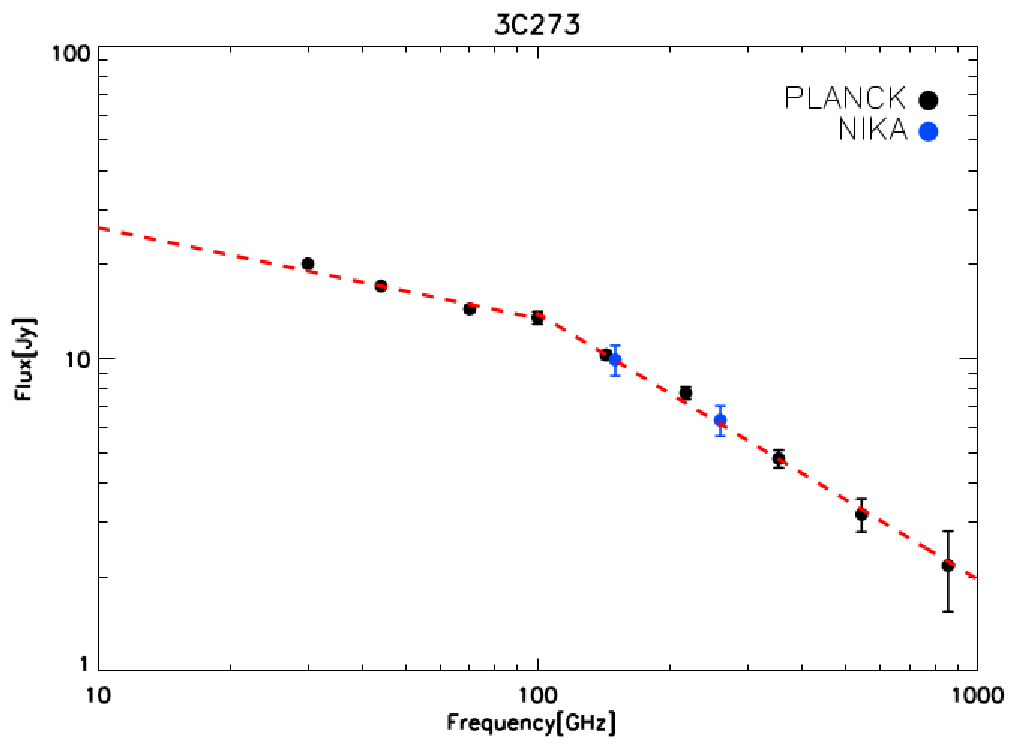
\includegraphics[%
  % width=0.66\linewidth,keepaspectratio]{figures/ALMA_PLANCK_sed2_3C273.pdf}
  % \caption{ 3C 273 spectral energy density (SED) of PLANCK and {\it NIKA} .}
  % \label{sed_3C273}
 % \end{center}
  % \end{figure}
   
 % Instrumental polarization and results ------------------------------------------------------------------------     
 
 %\section{Polarimetry calibration}\label{polcalib}
 
 
 %In order to give an example on a polarized source we show the maps obtained for the quasar 3C 273 in Fig. ~ \ref{3c273_ex}. In this figure we show the maps before applying the algorithm of correction (left column) and after (right column); the efficiency of this correction allows us to estimate a more correct polarization degree and angle. Here the quasar is taken as example but a proper discussion on the results obtained in terms of polarization degree and angle is given in the calibration section. 
 
 
 
 
 %\subsubsection{Parallel session {\it NIKA} - XPOl}
 %On February 2015 we performed an observational parallel session with XPOl experiment. In this section we will discuss the results obtained by the data analysis from the two experiments. 
 %The results of this parallel session of the observations done between {\it NIKA} and XPOl are shown in Tab. \ref{tab:calib_degree}. 
 
 %As Faraday rotation is proportional to $\lambda^2$  \citep{mckee} Faraday rotation measures (RMs) are expected to diminish at high frequencies. The core of the 3C273 shows this trend \citep{Attridge} at 86 GHz and explains the XPOl results. 
 
 %There are some differences and incompatibilities between {\it NIKA} and XPOl data, most of them are likely due to expected trends between the different wavelengths of the instruments. At higher frequencies closer to the base of the jet the magnetic field tends to be more ordered. This can be explain why the polarization degree tends to increase towards higher frequency. 
 
 %The polarization angle is mainly affected by Faraday rotation which changes the angle as proportional $\lambda^2$. It is a weak effect at mm wavelengths, but clearly present in the more active AGNs. This affects more the 3 mm than 2 and 1 mm data. 
 
 %An other effect must also be expected due to changing optical depth with frequency which allows to see different parts of the jet where the magnetic field (and thus the polarization angle) may be different. 
 
 %As Faraday rotation is proportional to $\lambda^2$  \citep{mckee} Faraday rotation measures (RMs) are expected to diminish at high frequencies. The core of the 3C273 shows this trend \citep{Attridge} at 86 GHz and explains the XPOl results. 
 
 %{\it NIKA} polarimeter measures {$\psi$} = (-89.3 $\pm$ 3.2)$^\circ$ and $\psi$ = (-74.1 $\pm$ 3.9)$^\circ$, $p$ = [3.8$\pm$0.4] $\%$ and $p$=[2.0 $\pm$ 0.5] $\%$ at 260 GHz and 150 GHz, respectively. 
 
 %XPOl measures {$\psi$} = (-76.8 $\pm$ 1.6)$^\circ$  and {$\psi$} = (-37.8 $\pm$ 0.9)$^\circ$, $p$ = [3.6$\pm$0.2] $\%$ and $p$ = [1.1$\pm$0.0] $\%$ at 229 GHz and 86 GHz, respectively.
 
 %This is the strongest source that we observed in parallel with XPOl and there is agreement between two experiments in both polarization degree and angle.
 
 %For the quasar 0851+202 there is a clear discrepancy in the angles between instruments for which we do not have an explanation. May be we have to check in the next observations. There is an agreement for both {\it NIKA} wavelengths.
 
 %For the quite variable quasar 1749+096 the {\it NIKA} 1 mm polarization degree is higher than XPOl that observes at 229 GHz.
 
 %The quasar 0415+379 is the weakest source at 1mm and however quite variable. It is too weak for XPOl measurement, we observe however an agreement between the two mm channel of {\it NIKA}.
 
 
 % Extended sources section --------------------------------	
 %OMC-1
  \begin{figure*}
   \begin{center}
   \includegraphics[%
   width=0.33\linewidth,keepaspectratio]{figures/CYGNUSA_I_map.eps}
    \includegraphics[%
   width=0.33\linewidth,keepaspectratio]{figures/CYGNUSA_Q_map.eps}
    \includegraphics[%
   width=0.33\linewidth,keepaspectratio]{figures/CYGNUSA_U_map.eps}
    \includegraphics[%
   width=0.33\linewidth,keepaspectratio]{figures/CYGNUSA_I_map_2mm.eps}
    \includegraphics[%
   width=0.33\linewidth,keepaspectratio]{figures/CYGNUSA_Q_map_2mm.eps}
    \includegraphics[%
   width=0.33\linewidth,keepaspectratio]{figures/CYGNUSA_U_map_2mm.eps}
    \caption{Cygnus~A Stokes $I$, $Q$ and $U$ maps  at 260 GHz %leakage corrected $I$, $Q$ and $U$ maps  at 260 GHz
      (top) and 150 GHz (bottom). The $Q$, $U$ maps are smoothed with a Gaussian filter of 6 arcsecond. At 260 GHz the $I$ map is also smoothed 
      to 4 arcsecond for display purposes. The effective beam FWHM is shown as a white circle
      in the bottom left corner of each panel. The contours in $Q$ and $U$ represent the intensity map for
      each frequency. They start from 0.2 Jy/beam with steps of 0.2
      Jy/beam. Polarization vectors are plotted in red in the intensity image when $I$ $>$ 0 and $P > 2\sigma_P$.}
     \label{cygnusa_maps}
   \end{center}
   \end{figure*}
   

 \begin{figure*}
   \begin{center}
   \includegraphics[%
   width=0.33\linewidth,keepaspectratio]{figures/M87_I_map.eps}
    \includegraphics[%
   width=0.33\linewidth,keepaspectratio]{figures/M87_Q_map.eps}
    \includegraphics[%
   width=0.33\linewidth,keepaspectratio]{figures/M87_U_map.eps}
    \includegraphics[%
   width=0.33\linewidth,keepaspectratio]{figures/M87_I_map_2mm.eps}
    \includegraphics[%
   width=0.33\linewidth,keepaspectratio]{figures/M87_Q_map_2mm.eps}
    \includegraphics[%
   width=0.33\linewidth,keepaspectratio]{figures/M87_U_map_2mm.eps}
    \caption{ \nika\ M87 Stokes  $I$, $Q$ and $U$ maps  at 260 GHz (top) and 150 GHz (bottom). 
    For display purposes, at 260 GHz the $Q$, $U$ maps are smoothed with a Gaussian filter of 6 arcsecond and the
      $I$ map of 4 arcsecond. At 150 GHz the $Q$, $U$ maps are also smoothed to 4 arcsecond, while the $I$ map is not smoothed. The contours in $Q$ and $U$ represent the intensity map, for each frequency, starting from 0.2 Jy/beam with steps of 0.2 Jy/beam. Polarization vectors are plotted in red in the intensity image when $I$ $>$ 0 and $P > 2\sigma_P$.}
     \label{M87_maps}
   \end{center}
   \end{figure*}
   
    \begin{figure*}
   \begin{center}
     \includegraphics[%
   width=0.33\linewidth,keepaspectratio]{figures/Orion_I_map.eps}
     \includegraphics[%
   width=0.33\linewidth,keepaspectratio]{figures/Orion_Q_map.eps}
    \includegraphics[%
   width=0.33\linewidth,keepaspectratio]{figures/Orion_U_map.eps}
      \includegraphics[%
   width=0.33\linewidth,keepaspectratio]{figures/Orion_I_map_2mm.eps}
     \includegraphics[%
   width=0.33\linewidth,keepaspectratio]{figures/Orion_Q_map_2mm.eps}
    \includegraphics[%
   width=0.33\linewidth,keepaspectratio]{figures/Orion_U_map_2mm.eps}
 \caption{ {\it NIKA} Stokes $I$, $Q$ and $U$ maps of Orion
   OMC-1 at 260 GHz (top) and 150 GHz (bottom). The intensity contours over-plotted in the
   $Q$ and $U$ maps corresponds to (1, 2, 6, 10, 20, 38) Jy/beam at 260 GHz and
   (2, 4, 6, 8, 10, 14) Jy/beam at 150 GHz. Polarization vectors are plotted in black in the intensity image when $I$ $>$ 0 and $P$ $> 2\sigma_P$.}
   \label{Orion}
   \end{center}
   \end{figure*}
      \begin{figure}
  \caption{ Polarization intensity (a), degree (b) and angle (c) maps of Orion Molecular Cloud (OMC-1) at 260 GHz (left) and 150 GHz (right) with intensity contours over-plotted. Only the regions with P > 2 $\sigma_P$ are plotted on (b) and (c). At both frequencies, for display purposes, the polarization intensity maps are smoothed with a Gaussian filter of 6 arcsecond; while the polarization degree and angle maps are smoothed to 2 arcsecond.}
     \begin{center}
  	\setlength{\unitlength}{\columnwidth} 
\begin{picture}(2,2.5)
 \put(0,2.5){(a)}
           \put(0.05,2.05) { \includegraphics[%
   width=0.4\linewidth,keepaspectratio]{figures/Orion_ipol_1mm.eps}}
      \put(0.5,2.05){ \includegraphics[%
   width=0.4\linewidth,keepaspectratio]{figures/Orion_ipol_2mm.eps}}

    \put(0,2.0){(b)}
   
      \put(0.05,1.55){  \includegraphics[width=0.4\linewidth,keepaspectratio]{figures/Orion_poldeg_1mm.eps}}
	\put(0.5,1.55){\includegraphics[width=0.4\linewidth,keepaspectratio]{figures/Orion_poldeg_2mm.eps}}
	
     \put(0,1.5){(c) }
   
    \put(0.05,1.05){\includegraphics[%
   width=0.4\linewidth,keepaspectratio]{figures/Orion_angle_1mm.eps}}
    \put(0.5,1.05){\includegraphics[%
   width=0.4\linewidth,keepaspectratio]{figures/Orion_angle_2mm.eps}}
	\end{picture}
 \end{center}
\label{Orion_poldeg}
  \end{figure}
  
  \begin{figure*}
    \begin{center}
     \includegraphics[%
   width=0.8\linewidth,keepaspectratio]{figures/Column_density_Orion.png}
    \caption{Column density map (left) obtained by the intensity map $I$ at 1.15 mm. For comparison the polarization fraction is reported on the right panel of the figure.}
    \label{column_density}
\end{center}
  \end{figure*}
  
 \section{\nika\ polarized observations of compact and extended sources}
 \label{sec:extended}
 We discuss here observations of compact and extended polarized sources, which
 allow us to further validate the quality of the reconstruction of the polarized
 sky signal with the \nika\ camera. Special care is taken on the verification of
 the validity of the leakage correction algorithm, which can affect the
 reconstruction of the direction of polarization across the source. We have
 performed observations of different types of sources: Cygnus~A, a radio galaxy
 with diffuse emission between the two radio lobes; M87, an external galaxy; and Orion OMC1, a nearby highly polarized galactic cloud. Observations of the Crab nebula have been performed several times
 during the \NIKA\ polarization runs. 
 A preliminary report on these observations has been given in \citep{Ritacco2015}.
 A full astrophysical study of the Crab nebula ({\it in prep.}) is beyond the scope of this paper.

\subsection{Cygnus~A}
Cygnus~A is a typical radio galaxy with twin jets of plasma emanating from its
nucleus and forming two extended, radio lobes. Cygnus~A is the most
powerful Fanaroff- Riley II (FRII) radio galaxy in the local environment. It has
been well studied in terms of spatial resolution as it lies at a distance of 227
Mpc. At low radio frequencies, the synchrotron emission from the two giant lobes
\nico{dominates} \citep{1974MNRAS.166..305H}. At higher frequencies the hotspots
(working surfaces in the lobes) and the galaxy core become more prominent. The
southern and northern hotspots are at 50 and 70 arcsec from the core,
respectively.  The complex structure of Cygnus~A can be well explained by
assuming that it consists of two components, which are polarized in opposite
directions and of an unpolarized core \cite{1967ApJ...150L..15S},
\cite{1966SvA....10..214S}, \cite{1968ApJ...151...53M}.
 
The \nico{**} \nika\ Stokes $I$, $Q$, and $U$ maps of Cygnus~A at 260
(top row) and 150 (bottom row) GHz are presented in Fig.~\ref{cygnusa_maps}.
On the intensity maps the polarization vectors are over-plotted in red. On the
$Q$ and $U$ maps intensity contours are also represented in red.  As expected,
on the intensity maps at 1.15 and 2.05 mm we clearly observe three compact
sources that correspond to the core and the two hotspots. By contrast, the
polarization maps show only two polarized regions that correspond to the hotspots and nothing on the core. This is an unambiguous confirmation of the
astrophysical origin of the observed polarization: if it was due to the instrumental
polarization, it would be proportional to the total intensity (and therefore show up
on the core) and with identical direction on the entire map. Such considerations
are further confirmed on other extended sources as presented in the next sections.
\subsection{M87}
 M87, also designated as 3C274, or NGC 4486, or Virgo A, is a giant elliptical
 galaxy \citep{dev76} located near the core of the Virgo cluster.  Its nucleus is
 a radio and X-ray source from which emanates an optical jet.  M87 is
 estimated to be about 16 Mpc from Earth \citep{mou80}. The core and
 the jet can be seen at all wavelengths from radio to X-rays.
 %Radio galaxies serve as a probe of their environments, providing means
 %to study the pressure, density, temperature, and magnetic strength, {\it
 %etc.} of the extragalactic medium (IGM) or intra-cluster
 %medium (ICM). 
 %The galaxy M87 is more studied at lower frequencies than the {\it NIKA} ones in order to study the physics of the filaments, the polarization 
 %degrees of the filaments are very high near the limit of synchrotron 
 %emission at this frequencies. At {\it NIKA} frequencies the galaxy appears with its core and the surrounding lobes. 
 Fig.~\ref{M87_maps} presents the \nika\ \nico{**} Stokes $I$, $Q$ and
 $U$ maps at 260 (top) and 150 (bottom) GHz. The polarization vectors are
 over-plotted in red on the intensity maps representing both the degree and
 orientation of polarization. The peak surface brightness of the $I$ map is $\sim$ 0.6 Jy/beam
and $\sim$ 1.5 Jy/beam at 260 GHz and 150 GHz, respectively. This confirms the fact
 that the M87 emission is dominated by synchrotron. The polarization vectors are
 well aligned following the intensity contours. They suggest the
 existence of a large scale ordered magnetic field in the radio lobes of M87.
 %The polarized intensity at 150 GHz shown in Fig.~\ref{M87_ipol} suggests a synchrotron emission of the M87 lobes.  The polarized emission at 260 GHz is quite weak. 
 % Fig.~\ref{m87_vector} show the Stokes vector $I$ with the vectors indicating the orientation of the polarization angle at both frequencies.  T
 %The hot spots present a spectral index (right map on the row) in
 %the range -1.5 to -2.0, which is consistent with synchrotron emission but
 %steeper than the value found by \citet{1998MNRAS.301..935R}, which is $\sim
 %-1$. The galaxy core shows a flatter spectrum from -0.6 to -1.0, which is
 %consistent with previous estimates from \citet{1999IAUS..194..179L}.

\subsection{Orion OMC-1}
The Orion Molecular Cloud (OMC-1) is the closest site of OB star formation. The
Nebula (KL) is the flux peak from far infrared to millimeter wavelengths on the
OMC-1 ``ridge" \citep{schle1998}.  A sub-millimeter peak (KHW) with equal mass
but lower dust temperature, is found 90 arcsec south of KL along the ridge
\citep{KHW1982}. At KL and KHW, the polarization fraction increases with the
wavelength \citep{schle1998}.

Fig.~\ref{Orion} presents the \nika\ \nico{**} Stokes $I$, $Q$ and $U$ maps of
Orion OMC-1 at 260 (top) and 150 (bottom) GHz.  Polarization vectors are
over-plotted on the intensity maps, showing both the polarization degree and
orientation.  The peak surface brightness of the OMC-1 emission is about 45.8
Jy/beam and 14 Jy/beam at 260 GHz and 150 GHz, respectively. The size of the map
is 8 $\times$ 8 arcminutes and it is obtained by the co-addition of 18 maps for
a total observational time of about 5h.  The left panel of
Fig.~\ref{column_density} shows the column density map obtained by the continuum
emission of Orion OMC-1 observed at 1.15 mm. Mostly driven by our sensitivity
limit, polarization is only detected at column densities > 4 $\times$ 10$^{23}$
cm$^{-2}$ in the map.  Depolarization is observed at column densities > 2
$\times$ 10$^{24}$ cm$^{-2}$ at 1.15 mm, while the 2.05 mm polarized fluxes
seems less sensitive to depolarization.

The orientation of the polarization vectors is consistent between the 260 and
150 GHz maps, confirming the same physical origin of the observed polarization.
\nico{We observe} a very organized magnetic field topology with field lines
mostly oriented to the integral-shaped filament, and suggesting some bending of
the field lines along the major axis of the filament towards the high column
density cores, maybe due to the field lines being dragged by large-scale
converging material accreting along the filament onto the cores.  These
structures and filaments are consistent with OMC-1 observations performed with
SCUPOL \citep{scubapol} at 850 $\mu$m.  Previous observations at 1.3 mm
performed by \cite{leach1991} show that at the KL position, the average
polarization rises to 4\%-5\% while at KL, the polarization drops to 0.6\%.

The polarization intensity maps $P$ are reported on the top panel of Fig.~\ref{Orion_poldeg} (a), showing the expected ``polarization hole'' across the KL nebula, already observed by \cite{schle1998}. The polarization degree maps $p$ as observed at both \NIKA\ frequencies are reported on the central panel of Fig.~\ref{Orion_poldeg} (b).
We observe on both maps a polarization degree that reaches a level of about 10\% of the total intensity in regions where the diffuse intensity emission is observed. This polarization fraction decreases greatly near the KL nebula.
The polarization angle $\psi$ is shown on the bottom panel of Fig.~\ref{Orion_poldeg} (c). It shows up approximately constant on the extended emission reaching a value of $\sim$ 20-30$^{\circ}$.  Averaging across the KL nebula on the \nika\ Orion
maps at 260 GHz (1.15 mm) we find that the angle and degree of polarization are
$\psi$ = (37.74 $\pm$ 3.56)$^\circ$ and $p$ = (0.6 $\pm$ 0.2) $\%$.  
The uncertainties reported here are purely statistical. We have also to consider the systematic
uncertainties due to HWP zero position 1.8$^{\circ}$ as well as the absolute calibration error calculated on Uranus, about $\sim$14\% at 260 GHz and 5\% at 150 GHz.
%Then, for the KHM region we find $\psi$ = (18.7 $\pm$ 0.7)$^\circ$ and $p$ = (4.6 $\pm$1.2) $\%$. 
In Tab.~\ref{tab:tab_orion_polka_scupol} we summarize the results obtained on the KL region
by SCUPOL and POLKA experiments
for comparison with \nika\ results.
\begin{table*}
 \centering
 \caption{Summary on KL nebula polarisation degree and angle results obtained by previous experiments and \nika. An absolute uncertainty of 1.8$^{\circ}$ has to be added to the statistical angle uncertainties reported here.}
 \footnotesize
 \begin{tabular}{cccccccccccc}
 \hline
 \hline
  \multicolumn {3} {c} {p [$\%$]} & \multicolumn {3} {c} {$\psi$ [$^\circ$]} \\
 \hline
 POLKA  & SCUPOL  &  \nika\  & POLKA  & SCUPOL   &  \nika\ \\
  \hline
   [870 $\mu$ m] &  [850 $\mu$ m]  &  [1.15 - 2.05 mm]  &  [870 $\mu$ m] &  [850 $\mu$ m]  &  [1.15 - 2.05 mm] \\
  \hline
  0.7 $\pm$ 0.2 & 0.7 $\pm$ 0.1 & (0.6 $\pm$ 0.2) - (1.0 $\pm$ 0.2) &  32.8 $\pm$ 7.6 & 40.8 $\pm$ 5.4 & [37.73 $\pm$ 3.56] - [25.35 $\pm$ 2.15] \\ 
 \hline
 \hline
 \end{tabular}
 \label{tab:tab_orion_polka_scupol}
 \end{table*}    
 %$\psi$ = [19.07 $\pm$ 1.15(stat) $\pm$ 1.8(syst)]$^\circ$ and $p$ = (2.6 $\pm$ 0.1) $\%$ at 150 GHz. 
 %At the KHM region we find $\psi$ = (18.7 $\pm$ 0.7 stat) $\pm$ 1.8(syst)) $^\circ$ and $p$ = (4.6 $\pm$ 0.2) $\%$ and $\psi$ = [18.0 $\pm$ 0.6 stat) $\pm$ 1.8(syst)]$^\circ$ and $p$ = (4.7 $\pm$ 0.2) $\%$ at 260 and 150 GHz, respectively.
 
 %The leakage maps found for this source represented in Fig.~\ref{Orion_leakage} show a reduced leakage effect compared to point source polarization degree. In Fig.~\ref{orion_vector} we show the Stokes vector $I$ with the vectors indicating the orientation of the polarization angle.
 %In Fig.~\ref{Orion_scuba} we show the maps of Orion OMC-1 obtained by SCUPOL instrument \citep{scubapol} at 850 $\mu$m. The contours represent the {\it NIKA} map obtained at 1.15 mm. We observe a bit shift between the two maps may be due to some pointing error in the specific observation session. 
 %If we compare the polarization intensity IPOL in Fig.~\ref{Orion_scuba} on right with the polarization intensity  $IPOL$ = $\sqrt{Q^2 + U^2}$ obtained by {\t NIKA} observation in Fig.~\ref{Orion_ipol} there is a consistency in the shape of the polarized regions. 
 %\begin{figure}
 %  \begin{center}
 %    \includegraphics[%
 %  width=1.\linewidth,keepaspectratio]{figures/NIKAvsScuba.pdf}
 %  \caption{ \NIKA\ Stokes $I$ at 260 GHz with SCUPOL map contours at 850 $\mu m$. The \NIKA\ map is shifted by $\sim$ 10 arcsec to match the SCUPOL map.}
 %  \label{Orion_scuba}
 %  \end{center}
  % \end{figure} 
  
  
 
\section{Conclusions}\label{conclusions}
This paper has presented the first \nico{astrophysical} polarization
measurements with KIDs. For these measurements we have adopted a simplified
polarization system consisting of an achromatic, continuously rotating HWP at
about 3~Hz, an analyzer, and arrays of KIDs not sensitive to polarization.  The
fast modulation of the input polarization signal with the HWP has allowed us to
significantly reduce the atmospheric emission in the polarized
signal. Instrumental polarization in the form of intensity to polarization
leakage \nico{with a non trivial point spread function} has been observed at the
level of 2 to 3\% peak to peak for point like and extended sources
respectively. We have successfully developed an algorithm to correct for this
systematic effect {\nico, up to a residual instrumental polarization directly
  proportionnal to $I$ at the level of} 0.7\% and 0.6\% at 1.15 and 2.05~mm
respectively, that is straightforward to correct.  We have observed 3C286, a
quasar used as \nico{a} standard polarization calibrator in literature and we
have found a total flux, a polarization degree and orientation in agreement with
existing data. These results have been confirmed on other quasars such as 3C279,
3C273, 0923+392 for which we either found comparison results in literature or
performed simultaneous measurements with XPOL. We have also observed compact and
extended sources such as Cygnus~A, OMC-1 and M87, and again, found consistent
results with existing polarization maps at about the same wavelength ({\it e.g.}
OMC-1 \cite{scubapol}). All these observations establish the accuracy of our
system and analysis on astronomical sources with fluxes of about one Jansky and
degrees of polarization as low as 3\%. \nico{On extended sources such as OMC-1,}
\nika\ observations confirm that \nico{polarization} vectors align well with the intensity
structures indicating the presence of well ordered magnetic fields. To our
knowledge, our observations of Cygnus~A and M87 are the first ones in
polarization at millimetric \nico{wavelengths} and the different orientation of
polarization in the two radio lobes of Cygnus~A is a striking feature,
\nico{already known in the literature, e.g.~\citet{1967ApJ...150L..15S}.}
\nika\ has been a successful test-bench for the
\nikad \footnote{http://ipag.osug.fr/nika2} camera, which shares the same
polarization system, but limited to the 260~GHz channel. \nikad\ will observe
the sky at the same frequencies with ten times more detectors and a FOV of 6.5
arcminutes. The \nikad\ camera has been installed at the IRAM 30 meter telescope
in Spain on October 2015 to start its commissioning phase for unpolarized
observations. A polarization dedicated commissioning will follow, during which
we will improve our understanding of the observed instrumental polarization and
our ability to correct for it.

This paper shows the potentialities of an instrument based on
KIDS and a fast and continuously rotating HWP to measure polarization, especially
from the ground where atmosphere is a nuisance, even more at low temporal
frequencies and large angular scales. It opens the way to forthcoming
observations with \nikad\ that will undoubtedly provide advances in the field of
Galactic emission and interactions with the magnetic field.
 
 \bibliography{biblio}
 % \begin{figure*}
 %  \begin{center}
 %   \includegraphics[%
 %    width=0.24\linewidth,keepaspectratio]{figures/Orion_IQ_1mm.pdf}
 %    \includegraphics[%
 %  width=0.24\linewidth,keepaspectratio]{figures/Orion_IU_1mm.pdf}
 %  \includegraphics[%
 %    width=0.24\linewidth,keepaspectratio]{figures/Orion_IQ_2mm.pdf}
 %    \includegraphics[%
 %  width=0.24\linewidth,keepaspectratio]{figures/Orion_IU_2mm.pdf}
 %  \caption{ From left to right Orion OMC-1 intensity to polarization leakage maps $IQ$, $IU$ at 260 GHz and at 150 GHz.}
 %  \label{Orion_leakage}
 %  \end{center}
 %  \end{figure*}
   
 
 %\begin{figure*}
 %  \begin{center}
 %        \includegraphics[%
 %  width=0.4\linewidth,keepaspectratio]{figures/Orion_ipol_1mm.pdf}
 %     \includegraphics[%
 %  width=0.4\linewidth,keepaspectratio]{figures/Orion_ipol_2mm.pdf}
 %     \caption{ polarization intensity maps at 260 GHz (left) and 150 GHz (right) of the molecular cloud Orion OMC-1. }
 %    \label{Orion_ipol}
 %  \end{center}
 %  \end{figure*}
 
 
 
  % M87
   
     
   % \begin{figure*}
  % \begin{center}
   % \includegraphics[%
   %  width=0.24\linewidth,keepaspectratio]{figures/M87_IQ_1mm.pdf}
    % \includegraphics[%
   %width=0.24\linewidth,keepaspectratio]{figures/M87_IU_1mm.pdf}
   %\includegraphics[%
  %   width=0.24\linewidth,keepaspectratio]{figures/M87_IQ_2mm.pdf}
    % \includegraphics[%
  % width=0.24\linewidth,keepaspectratio]{figures/M87_IU_2mm.pdf}
   %\caption{ From left to right M87 intensity to polarization leakage maps $IQ$, $IU$ at 260 GHz and at 150 GHz.}
   %\label{M87_leakage}
  % \end{center}
  % \end{figure*}
   
   %\begin{figure*}
   %\begin{center}
   %\includegraphics[%
  % width=0.48\linewidth,keepaspectratio]{figures/M87_ipol_1mm.pdf}
  % \includegraphics[%
  % width=0.48\linewidth,keepaspectratio]{figures/M87_ipol_2mm.pdf}
   %  \caption{ M87 polarization intensity maps at 260 GHz (left) and 150 GHz (right). }
    %   \label{M87_ipol}
   %\end{center}
   %\end{figure*} 
  
   % Cygnusa
   
 
   
  %  \begin{figure*}
  % \begin{center}
  % \includegraphics[%
  %  width=0.24\linewidth,keepaspectratio]{figures/Cygnus_A_IQ_1mm.pdf}
  %   \includegraphics[%
  % width=0.24\linewidth,keepaspectratio]{figures/Cygnus_A_IU_1mm.pdf}
  %\includegraphics[%
  %   width=0.24\linewidth,keepaspectratio]{figures/Cygnus_A_IQ_2mm.pdf}
  %   \includegraphics[%
  % width=0.24\linewidth,keepaspectratio]{figures/Cygnus_A_IU_2mm.pdf}
  % \caption{ From left to right Cygnus A intensity to polarization leakage maps $IQ$, $IU$ at 260 GHz and at 150 GHz.}
  % \label{cygnusa_leakage}
 %  \end{center}
 %  \end{figure*}
   
 %  \begin{figure*}
 %  \begin{center}
 %  \includegraphics[%
 %  width=0.48\linewidth,keepaspectratio]{figures/Cygnus_ipol_1mm_NIKA.pdf}
 %  \includegraphics[%
 %  width=0.48\linewidth,keepaspectratio]{figures/Cygnus_ipol_2mm_NIKA.pdf}
 %   \caption{ Cygnus A polarization intensity maps at 260 GHz (left) and 150 GHz (right). }
 %      \label{cygnusa_ipol}
 %  \end{center}
 %  \end{figure*} 
  
   % Projection of vectors------------------
   
 % \begin{figure*}
 %  \begin{center}
 %  \includegraphics[%
 %  width=0.42\linewidth,keepaspectratio]{figures/map_I_1mm_vector_M87.pdf} 
 %  \includegraphics[%
 %  width=0.42\linewidth,keepaspectratio]{figures/map_I_2mm_vector_M87.pdf} 
 %    \caption{ M87 Stokes vector $I$ intensity with polarization vectors at 260 GHz (left) and 150 GHz (right).}
 %  \label{m87_vector}
 %   \end{center}
 %  \end{figure*}
 
 %\begin{figure*}
 %  \begin{center}
 %  \includegraphics[%
 %  width=0.42\linewidth,keepaspectratio]{figures/Cygnusa_map_I_1mm_vector.pdf} 
 %  \includegraphics[%
 %  width=0.42\linewidth,keepaspectratio]{figures/Cygnusa_map_I_2mm_vector.pdf} 
 %    \caption{ Cygnus A Stokes vector $I$ intensity with polarization vectors at 260 GHz (left) and 150 GHz (right).}
 %	\label{cygnusa_vector}
 %   \end{center}
 %  \end{figure*}
 
  
   
   %-----------------------------------------------------
 \begin{acknowledgements}
We would like to thank the IRAM staff for their support during the campaigns. 
The NIKA dilution cryostat has been designed and built at the Institut N\'eel. 
In particular, we acknowledge the crucial contribution of the Cryogenics Group, and 
in particular Gregory Garde, Henri Rodenas, Jean Paul Leggeri, Philippe Camus. 
This work has been partially funded by the Foundation Nanoscience Grenoble, the LabEx FOCUS ANR-11-LABX-0013 and 
the ANR under the contracts "MKIDS", "NIKA" and ANR-15-CE31-0017. 
This work has benefited from the support of the European Research Council Advanced Grant ORISTARS 
under the European Union's Seventh Framework Programme (Grant Agreement no. 291294).
We acknowledge fundings from the ENIGMASS French LabEx (R. A. and F. R.), 
the CNES post-doctoral fellowship program (R. A.),  the CNES doctoral fellowship program (A. R.) and 
the FOCUS French LabEx doctoral fellowship program (A. R.).
\end{acknowledgements}
 
 %\pagebreak

        
\end{document}
